\documentclass{article}
\pdfoutput=1

% if you need to pass options to natbib, use, e.g.:
%     \PassOptionsToPackage{numbers, compress}{natbib}
% before loading neurips_2019

% ready for submission
\usepackage[final, nonatbib]{neurips_2019}
\usepackage{amsfonts}
\usepackage{amsmath}
\usepackage{amsthm}
\usepackage{amssymb}
\usepackage{graphicx}
\usepackage{caption}
\usepackage{subcaption}
\usepackage{xcolor}
\usepackage[utf8]{inputenc}
\usepackage{thmtools, thm-restate}
\usepackage[normalem]{ulem}
% \usepackage{xpatch}
% \usepackage{apptools}

% \makeatletter
% \xpatchcmd{\thmt@restatable}% Edit \thmt@restatable
% {\csname #2\@xa\endcsname\ifx\@nx#1\@nx\else[{#1}]\fi}% Replace this code
% {\IfAppendix{\csname #2\@xa\endcsname}{\csname #2\@xa\endcsname\ifx\@nx{Restatement}\@nx\else[{Restatement}]\fi}}% with this code
% {}{} % execute code for success/failure instances
% \makeatother

\newtheorem{theorem}{Theorem}[section]
\newtheorem{lemma}[theorem]{Lemma}
\newtheorem{definition}[theorem]{Definition}
\newtheorem{example}[theorem]{Example}
\newtheorem{proposition}[theorem]{Proposition}
\newtheorem{corollary}[theorem]{Corollary}

\def\shownotes{1}  \ifnum\shownotes=0
\newcommand{\authnote}[2]{$\ll$\textsf{\footnotesize #1 notes: #2}$\gg$}
\else
\newcommand{\authnote}[2]{}
\fi
\newcommand{\tnote}[1]{{\color{blue}\authnote{Tengyu}{#1}}}



%\newcommand{\pl}[1]{}
%\newcommand{\tm}[1]{}
%\newcommand{\ak}[1]{}

\newcommand{\pl}[1]{\textcolor{red}{[PL: #1]}}
\newcommand{\pldel}[1]{\sout{\textcolor{red}{#1}}}
\newcommand{\tm}[1]{\textcolor{blue}{[TM: #1]}}
\newcommand{\ak}[1]{\textcolor{brown}{[AK: #1]}}

\newcommand{\expect}[0]{\ensuremath{\mathbb{E}}}
\newcommand{\prob}[0]{\ensuremath{\mathbb{P}}}
\newcommand{\ourcal}[0]{the scaling-binning calibrator}
\newcommand{\Ourcal}[0]{The scaling-binning calibrator}

\graphicspath{ {images/} }

% to compile a preprint version, e.g., for submission to arXiv, add add the
% [preprint] option:
%     \usepackage[preprint]{neurips_2019}

% to compile a camera-ready version, add the [final] option, e.g.:
    %  \usepackage[final]{neurips_2019}

% to avoid loading the natbib package, add option nonatbib:
%     \usepackage[nonatbib]{neurips_2019}

\usepackage[numbers]{natbib}
\usepackage[utf8]{inputenc} % allow utf-8 input
\usepackage[T1]{fontenc}    % use 8-bit T1 fonts
\usepackage{hyperref}       % hyperlinks
\usepackage{url}            % simple URL typesetting
\usepackage{booktabs}       % professional-quality tables
\usepackage{amsfonts}       % blackboard math symbols
\usepackage{nicefrac}       % compact symbols for 1/2, etc.
\usepackage{microtype}      % microtypography

\newcommand{\argmax}{\mathop{\mbox{argmax}}}
\newcommand{\argmin}{\mathop{\mbox{argmin}}}
\newcommand{\argsup}{\mathop{\mbox{argsup}}}
\newcommand{\bins}{\mathcal{B}}

\title{Verified Uncertainty Calibration}

% The \author macro works with any number of authors. There are two commands
% used to separate the names and addresses of multiple authors: \And and \AND.
%
% Using \And between authors leaves it to LaTeX to determine where to break the
% lines. Using \AND forces a line break at that point. So, if LaTeX puts 3 of 4
% authors names on the first line, and the last on the second line, try using
% \AND instead of \And before the third author name.

% \setcounter{footnote}{0}
% \renewcommand*{\thefootnote}{\fnsymbol{footnote}}

\author{%
  Ananya Kumar, Percy Liang, Tengyu Ma \\
  Department of Computer Science\\
  Stanford University\\
  \texttt{\{ananya, pliang, tengyuma\}@cs.stanford.edu} \\
  % examples of more authors
  % \And
  % Percy Liang \\
  % Department of Computer Science\\
  % Stanford University\\
  % \texttt{pliang@cs.stanford.edu} \\
  % \And
  % Tengyu Ma \\
  % Department of Computer Science\\
  % Stanford University\\
  % \texttt{tengyuma@stanford.edu} \\
}

\begin{document}

\maketitle

\begin{abstract}
  Applications such as weather forecasting and personalized medicine demand models that output calibrated probability estimates---those representative of the true likelihood of a prediction. Most models are not calibrated out of the box but are recalibrated by post-processing model outputs. We find in this work that popular recalibration methods like Platt scaling and temperature scaling are (i) less calibrated than reported, and (ii) current techniques cannot estimate how miscalibrated they are. An alternative method, histogram binning, has measurable calibration error but is sample inefficient---it requires $O(B/\epsilon^2)$ samples, compared to $O(1/\epsilon^2)$ for scaling methods, where $B$ is the number of distinct probabilities the model can output. To get the best of both worlds, we introduce \emph{\ourcal{}}, which first fits a parametric function that acts like a baseline for variance reduction and then bins the function values to actually ensure calibration. This requires only $O(1/\epsilon^2 + B)$ samples. We then show that methods used to estimate calibration error are suboptimal---we prove that an alternative estimator introduced in the meteorological community requires fewer samples ($O(\sqrt{B})$ instead of $O(B)$). We validate our approach with multiclass calibration experiments on CIFAR-10 and ImageNet, where we obtain a 35\% lower calibration error than histogram binning and, unlike scaling methods, guarantees on true calibration.

% Applications such as weather forecasting and personalized medicine demand models that output calibrated probability estimates---those representative of the true likelihood of a prediction.
% Scaling recalibration methods that fit a parametric model are great, because they require $O(1/\epsilon^2)$ samples to achieve calibration error $\epsilon$, but we find in this work that they are (i) less calibrated than reported and (ii) current techniques cannot estimate how miscalibrated they are.
% An alternative method, histogram binning, is sample inefficient -- it requires $O(B/\epsilon^2)$ samples where $B$ is the number of distinct probabilities the model can output.
% To solve these problems, we introduce the variance-reduced calibrator, which first fits a parametric function that acts like a baseline for variance reduction and then bins the function values to actually ensure calibration.
% This requires only $O(1/\epsilon^2 + B)$ samples.\tm{changed the order of two summands}
% We also show that the methods used in the machine learning literature to estimate calibration error are suboptimal -- we prove that an alternative estimator introduced in the meteorological community requires fewer samples -- samples proportional to $\sqrt{B}$ instead of $B$.
% We validate our approach with multiclass calibration experiments on CIFAR-10 and ImageNet, where we get a 2x lower calibration error than histogram binning and guarantees on true calibration unlike scaling methods.
% In this paper, we first show that previous calibration methods like Platt scaling and temperature scaling are (i) less calibrated than reported and (ii) we do not know how miscalibrated they are, because prior work only gives lower bounds for their calibration error \pl{reframe this: previous work (possibly some of our reviewers) did not think they were giving lower bounds; should say instead that methods used by previous work to assess calibration underestimate the true calibration error}.
%   Other methods \pl{what other methods?} like histogram binning are sample inefficient -- they require $O(\frac{B}{\epsilon^2})$ samples to reach calibration error $\epsilon$, where $B$ is the number of model outputs \pl{be clear: which model? this looks like you're talking about number of classes; which is coincidentally what you want, I guess!}. To solve these problems, we introduce the variance-reduced calibrator.
%   The variance-reduced calibrator first fits a parametric function -- which acts like a baseline for variance reduction -- and then bins the function values to actually ensure calibration. This requires only $O(B + \frac{1}{\epsilon^2})$ samples. \pl{we can join some sentences to make it flow better}
%   \pl{compress: We also introduce a new estimator for verifying...}
%   We then turn to the question of how to verify calibration. We introduce a new estimator for the calibration error that requires fewer samples -- samples proportional to $\sqrt{B}$ instead of $B$. We prove finite sample guarantees for all our results, and validate our theory with multiclass calibration experiments on CIFAR-10 and ImageNet, where we get a 2x lower calibration error than histogram binning. \pl{and guarantees on true calibration unlike scaling methods}
\end{abstract}

%\pl{Writing tip: find ways to group statements into single sentences so that you get some hierarchical structure: each sentence should express a set of related ideas, and important ideas are at the beginning of sentences}

\section{Introduction}

% Applications like personalized medicine, meteorological forecasting, and natural language processing \pl{NLP is so broad...anything could go here; either motivate based on fields that already use calibration (good to stand on shoulders of giants) or say something substantive about why calibration is needed (danger of being too preachy (danger of being too preachy))} require that classifiers provide calibrated confidence measures in addition to their predictions~\cite{jiang2012calibrating, brocker2009decomposition, nguyen2015posterior}.
% In other words, the probability that a system outputs for an event should reflect the true frequency of that event: if an automated diagnosis system says 1,000 patient have cancer with probability 0.1, approximately 100 of them should indeed have cancer.
The probability that a system outputs for an event should reflect the true frequency of that event: if an automated diagnosis system says 1,000 patients have cancer with probability 0.1, approximately 100 of them should indeed have cancer.
In this case we say the model is uncertainty calibrated. The importance of this notion of calibration has been emphasized in personalized medicine~\cite{jiang2012calibrating}, meteorological forecasting~\cite{murphy1973vector, murphy1977reliability, degroot1983forecasters,gneiting2005weather, brocker2009decomposition} and natural language processing applications~\cite{nguyen2015posterior, card2018calibration}.
As most modern machine learning models, such as neural networks, do not output calibrated probabilities out of the box~\cite{guo2017calibration, zadrozny2001calibrated, kuleshov2018accurate}, recalibration methods take the output of an uncalibrated model, and transform it into a calibrated probability.
\emph{Scaling} approaches for recalibration---Platt scaling~\cite{platt1999probabilistic}, isotonic regression~\cite{zadrozny2002transforming}, and temperature scaling~\cite{guo2017calibration}---are widely used and require very few samples, but do they actually produce calibrated probabilities?
% , and speech recognition~\cite{dong2011calibration}
% These methods use additional recalibration data to fit a simple function on top of the original model outputs.

% Important, check that it's not too similar to "On calibration of modern neural networks" paper.
% In many applications, classification models must not only be accurate, but should indicate when they may be incorrect. For example, in automated healthcare applications, control should be passed on to human doctors when the confidence of a disease diagnosis prediction is low. Specifically, classifiers should provide a \emph{calibrated} confidence measure in addition to its prediction. In other words, the probability that a system outputs for an event should reflect the true frequency of that event: of the times that a system says a patient has cancer with probability 0.3, 30\% of the time, the patient should indeed have cancer.
% Typically, complex models like neural networks do not output calibrated probabilities.
% Instead, recalibration methods take the output of an uncalibrated model, and transform it into a calibrated probability.
% Popular recalibration approaches include Platt scaling and temperature scaling.

% Recent advances in machine learning have dramatically increased predictive accuracy. Machine learning methods are now entrusted with making decisions in applications ranging from weather forecasting to medical diagnosis \pl{seems a bit naive...}. In many of these settings, classification models must not only be accurate, but should indicate when they may be incorrect. For example, in automated healthcare applications, control should be passed on to human doctors when the confidence of a disease diagnosis prediction is low. Specifically, classifiers should provide a \emph{calibrated} confidence measure in addition to its prediction. In other words, the probability that a system outputs for an event should reflect the true frequency of that event: of the times that a system says that it will rain with probability 0.3,  30\% of the time, it should rain.
% \pl{need citations; is rain prediction really driven by "modern ML"?}\tm{It also seems unncessary to introduce the rain example --- it seems to be a good introduction to people who didn't know it before, but not something to write in the first para of a paper?}

%  \pl{I'd try to combine with first paragraph so that it's all background}
% \pl{introduce calibration error as a central concern first;
% methods try to calibrate, but do they actually achieve it?
% }

\emph{We discover that these methods are less calibrated than reported.} Past work approximates a model's calibration error using a finite set of bins. We show that by using more bins, we can uncover a higher calibration error for models on CIFAR-10 and ImageNet.
We show that a fundamental limitation with approaches that output a continuous range of probabilities is that their true calibration error may never be measurable with a finite number of bins (Example~\ref{ex:continuous-not-calibrated}).

An alternative approach, histogram binning~\cite{zadrozny2001calibrated}, outputs probabilities from a finite set.
Histogram binning can produce a model that is calibrated, and unlike scaling methods we can measure its calibration error, but it is sample inefficient.
In particular, the number of samples required to calibrate scales linearly with the number of distinct probabilities the model can output, $B$~\cite{naeini2014binary}, which can be large particularly in the multiclass setting where $B$ typically scales with the number of classes.
Recalibration sample efficiency is crucial---we often want to recalibrate our models in the presence of domain shift~\cite{hendrycks2019anomaly} or recalibrate a model trained on simulated data, and may have access to only a small labeled dataset from the target domain.

To get the sample efficiency of Platt scaling and the verification guarantees of histogram binning, \emph{we propose the variance-reduced calibrator} (Figure~\ref{fig:var_red_binning}).
Like scaling methods, we fit a simple function $g \in \mathcal{G}$ to the recalibration dataset.
We then bin the input space so that an equal number of inputs land in each bin.
In each bin, we output the average of the $g$ values in that bin---these are the gray circles in Figure~\ref{fig:var_red_binning}.
In contrast, histogram binning outputs the average of the label values in each bin (Figure~\ref{fig:hist_binning}).
The motivation behind our method is that the $g$ values in each bin are in a narrower range than the label values, so when we take the average we incur less of an estimation error.
If $\mathcal{G}$ is well chosen, our method requires $O(\frac{1}{\epsilon^2} + B)$ samples to achieve calibration error $\epsilon$ instead of $O(\frac{B}{\epsilon^2})$ samples for histogram binning, where $B$ is the number of model outputs (Theorem~\ref{thm:final-calib}). Note that in prior work, binning the outputs of a function was used for evaluation and without any guarantees, whereas in our case it is used for the method itself and we show improved sample complexity.

% As with other recalibration methods, we begin with a recalibration dataset $\{(z_1, y_1), ..., (z_n, y_n)\}$, where $z_i$ represents the uncalibrated model output and $y_i$ the ground truth label.
% In the binary classification setting, $z_i \in [0, 1]$ and $y_i \in \{0, 1\}$.
% We fit a simple function $g \in \mathcal{G}$ to the recalibration dataset.
% We then bin the input space so that an equal number of $g(z_i)$ land in each bin.
% In each bin, we output the average of the $g(z_i)$ values in that bin -- these are the gray circles in Figure~\ref{fig:var_red_binning}.
% Binning ensures that the output probabilities are from a finite set, so we can check if it is calibrated.
% In contrast, histogram binning takes the average of the $y_i$ values in each bin (Figure~\ref{fig:hist_binning}).
% The motivation behind our method is that the $g(z_i)$ values in each bin are in a narrower range than the $y_i$ values -- when we take the average we incur less of an estimation error.
% If $\mathcal{G}$ is well chosen, our method requires $O(\frac{1}{\epsilon^2})$ samples to achieve calibration error $\epsilon$ instead of $O(\frac{B}{\epsilon^2})$ samples for histogram binning, where $B$ is the number of model outputs (Theorem~\ref{thm:final-calib}).
% \pl{this is good overall, but I wonder if it's too much setup / notation from the intro, and it's strange that it's introduced for our method and not the general problem setting}

\begin{figure}
     \centering
     \begin{subfigure}[b]{0.32\textwidth}
         \centering
         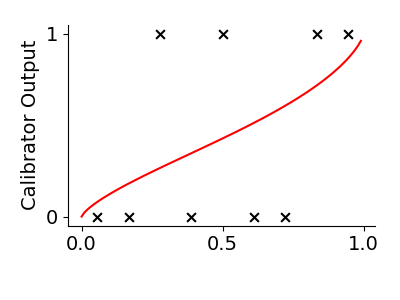
\includegraphics[width=\textwidth]{platt_scaling}
         \caption{Platt scaling.}
         \label{fig:platt_scaling}
     \end{subfigure}
     \hfill
     \begin{subfigure}[b]{0.32\textwidth}
         \centering
         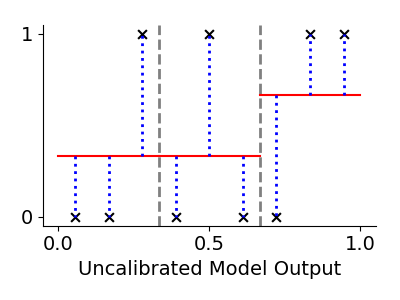
\includegraphics[width=\textwidth]{histogram_binning_with_deltas}
         \caption{Histogram binning.}
         \label{fig:hist_binning}
     \end{subfigure}
     \hfill
     \begin{subfigure}[b]{0.32\textwidth}
         \centering
         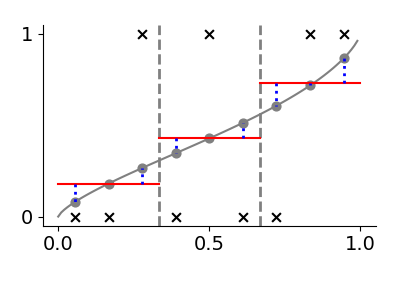
\includegraphics[width=\textwidth]{variance_reduced_binning_with_deltas}
         \caption{Variance-reduced calibrator.}
         \label{fig:var_red_binning}
     \end{subfigure}
        \caption{
        Visualization of the 3 recalibration approaches.
        The black crosses are the ground truth labels, and the red lines are the output of the recalibration methods.
        Platt Scaling (Figure~\ref{fig:platt_scaling}) fits a function to the recalibration data, but its calibration error is not measurable.
        Histogram binning (Figure~\ref{fig:hist_binning}) outputs the average label in each bin.
        Our variance-reduced calibrator (Figure~\ref{fig:var_red_binning}) fits a function $g \in \mathcal{G}$ to the recalibration data and then \emph{takes the average of the function values (the gray circles)} in each bin.
        The function values have lower variance than the labels, as visualized by the blue dotted lines, which is why our approach has lower variance. 
        }
        \label{fig:variance_reduced_illustration}
\end{figure}

Next, we turn to the question of estimating the calibration error. Prior work in machine learning~\cite{nguyen2015posterior, guo2017calibration, hendrycks2019anomaly, kuleshov2015calibrated, hendrycks2019pretraining} directly estimates each term in the calibration error from samples (Definition~\ref{dfn:plugin-estimator}). The sample complexity of this plugin estimator scales linearly with $B$. An alternative estimator introduced in the meteorological literature~\cite{brocker2012empirical, ferro2012bias} reduces the bias of the plugin estimator; \emph{we show that it has sample complexity that scales with $\sqrt{B}$}. We prove that it achieves this by leveraging error cancellations across bins.

We run multiclass calibration experiments on CIFAR-10~\cite{krizhevsky2009learningmultiple} and ImageNet~\cite{deng2009imagenet}.
The objective is to minimize the mean-squared error, also known as the Brier score~\cite{brier1950verification}, subject to a calibration error budget~\cite{gneiting2005weather}.
We show that the variance-reduced calibrator achieves a better calibration error than histogram binning, while allowing us to measure the true calibration error.
For example, we get a \emph{35\% lower calibration error on CIFAR-10} than histogram binning if $B = 100$.

% In summary, our contributions are:
% \begin{enumerate}
% \item We show that scaling methods for recalibration are less calibrated than reported.
% \item We propose variance-reduced calibration which has the sample complexity of scaling methods, but we can actually verify its calibration.
% \item We show that the method typically used to estimate calibration error is suboptimal, and an alternative estimator requires fewer samples to measure the calibration error.
% \end{enumerate}

\tm{Sometimes I do a summary of contribution paragraph for the reviewers to easily see the contribution. doesn't add anything to the quality of the paper, but sometimes useful for paper acceptance .. (As a rushed reviewer sometimes I wanted the authors to have a simple para with a bit more technical term than abstract....)}

\pl{it's a nice to have if we have space; the use of italics throughout the intro is actually pretty effective}


\section{Setup and background}
\label{sec:formulation}

\newcommand{\lpce}[0]{\ensuremath{\ell_p\mbox{-CE}}}
\newcommand{\ltwoce}[0]{\ensuremath{\ell_2\mbox{-CE}}}
\newcommand{\squaredce}[0]{\ensuremath{\ell_2^2\mbox{-CE}}}
\newcommand{\topsquaredce}[0]{\ensuremath{\ell_2^2\mbox{-TCE}}}
\newcommand{\margsquaredce}[0]{\ensuremath{\ell_2^2\mbox{-MCE}}}

\subsection{Binary classification}

Let $\mathcal{X}$ be the input space and $\mathcal{Y}$ be the label space where $\mathcal{Y} = \{0, 1\}$ in the binary classification setting.
Let $X \in \mathcal{X}$ and $Y \in \mathcal{Y}$ be random variables denoting the input and label, given by an unknown joint distribution $P(X, Y)$. Expectations are taken over all random variables unless otherwise specified.

Suppose we have a model $f : \mathcal{X} \to [0, 1]$ where the output of the model represents the model's confidence that the label is 1. As $f$ may not be calibrated, we define the calibration error, which examines the difference between the model's probability and the true probability given the model's output. If the calibration error is $0$ then the model is perfectly calibrated.

\begin{definition}[Calibration error]
For $p \geq 1$, the $\ell_p$ calibration error of $f : \mathcal{X} \to [0, 1]$ is given by:
\begin{align}
\lpce(f) = \Big(\expect\big[ \mid f(X) - \expect[Y \; | \; f(X)] \mid^p \big] \Big)^{1/p}
\end{align}
\end{definition}

The $\ell_2^2$ calibration error~\cite{murphy1973vector,murphy1977reliability,degroot1983forecasters, nguyen2015posterior, hendrycks2019anomaly, kuleshov2015calibrated, hendrycks2019pretraining, brocker2012empirical} is most commonly used but the $\ell_1$ and $\ell_{\infty}$ calibration errors are also used in the literature~\cite{guo2017calibration, naeini2015obtaining, nixon2019calibration}.

Calibration alone is not sufficient: consider an image dataset containing $50\%$ dogs and $50\%$ cats.
If $f$ outputs $0.5$ on all inputs, $f$ is calibrated but not very useful.
We often also wish to minimize the mean-squared error---also known as the Brier score---as defined below.

\begin{definition}
The mean-squared error of $f : \mathcal{X} \to [0, 1]$ is given by $\mbox{MSE}(f) = \mathbb{E}[(f(X) - Y)^2]$.
\end{definition}

We often want to minimize the MSE subject to a calibration constraint~\cite{gneiting2005weather, gneiting2007probabilistic}. Of course, these are not orthogonal because $\mbox{MSE} = 0$ implies perfect calibration---in fact the MSE is the sum of the $\ell_2^2$ calibration error and a ``sharpness'' term~\cite{murphy1973vector,degroot1983forecasters, kuleshov2015calibrated}.

\subsection{Multiclass classification}

While calibration in binary classification is well-studied,
it's less clear what to do for multiclass, where multiple definitions abound, differing in their strength. In the multiclass setting, $\mathcal{Y} = [K]$, where $[K] = \{1, \dots, K\}$ and $f : \mathcal{X} \to [0, 1]^K$ outputs a confidence measure for each class in $[K]$.

\begin{definition}[Top-label calibration error]
The $\ell_2^2$ top-label calibration error examines the difference between the model's probability for its top prediction and the true probability of that prediction given the model's output:
\begin{align}
\topsquaredce(f) = \expect\Big[ \Big( \prob\big(Y = \argmax_{j \in [K]} f(X)_j \mid \max_{j \in [K]} f(X)_j\big) - \max_{j \in [K]} f(X)_j \Big)^2 \Big]
\end{align}
\end{definition}

We would often like the model to be calibrated on less likely predictions as well---imagine that a medical diagnosis system says there is a $50\%$ chance a patient has a benign tumor, a $10\%$ chance she has an aggressive form of cancer, and a $40\%$ chance she has one of a long list of other conditions. We would like the model to be calibrated on all of these predictions so we define the marginal calibration error which examines, \emph{for each class}, the difference between the model's probability and the true probability of that class given the model's output.

\begin{definition}[Marginal calibration error]
\label{dfn:marginal-ce}
Let $w_k \in [0, 1]$ denote how important calibrating class $k$ is, where $w_k = \prob(Y = k)$ if all classes are equally important. The $\ell_2^2$ marginal calibration error is:
\begin{align}
\margsquaredce(f) = \sum_{k = 1}^K w_k \mathbb{E}\big[ (f(X)_k - \prob(Y = k \mid f(X)_k))^2 \big]
\end{align}
\end{definition}

Note that prior works~\cite{guo2017calibration, hendrycks2019anomaly, hendrycks2019pretraining} often claim to perform multiclass calibration but only measure top-label calibration---\cite{nixon2019calibration} shows that temperature scaling~\cite{guo2017calibration} scores worse than vector scaling on a marginal calibration metric, even though it has lower top-label calibration error.
% In the Appendix we discuss other notions of multiclass calibration.

\pl{is marginal calibration standard terminology? makes sense when compared with joint, but sounds a bit strange in relation to top-label}

\ak{There isn't a standard terminology here that I am aware of. Nixon et al (came out a few weeks before neurips deadline) have a similar metric called static calibration error. Seems fairly concurrent to ours, and I prefer marginal.}

For notational simplicity, our theory focuses on the binary classification setting. We can transform top-label calibration into a binary calibration problem---the model outputs a probability corresponding to its top prediction, and the label represents whether the model gets it correct or not. Marginal calibration can be transformed into $K$ one-vs-all binary calibration problems where for each $k \in [K]$ the model outputs the probability associated with the $k$-th class, and the label represents whether the input belongs to the $k$-th class or not~\cite{zadrozny2002transforming}---this is analogous to how vector scaling~\cite{guo2017calibration} extends Platt scaling. We look at both top-label calibration and marginal calibration in our experiments. There are other notions of multiclass calibration, such as joint calibration~\cite{murphy1973vector, brocker2009decomposition} and event-pooled calibration~\cite{kuleshov2015calibrated}. The former is a stronger notion of multiclass calibration that requires the entire probability \emph{vector} to be calibrated---achieving joint calibration efficiently is an important direction for future research.


\subsection{Recalibration}

Since most machine learning models do not output calibrated probabilities out of the box~\cite{guo2017calibration, zadrozny2001calibrated} recalibration methods take the output of an uncalibrated model, and transform it into a calibrated probability. That is, given a trained model $f: \mathcal{X} \to \mathcal{Z}$, let $Z = f(X)$. We are given recalibration data $T = \{ (z_i, y_i) \}_{i=1}^n$ independently sampled from $P(Z, Y)$, and we wish to learn a recalibrator $g : \mathcal{Z} \to [0, 1]$ such that $g \circ f$ is well-calibrated.

\emph{Scaling methods}, for example Platt scaling~\cite{platt1999probabilistic}, output a function $\hat{g} = \argmin_{g \in \mathcal{G}} \sum_{(z, y) \in T} \ell(g(z), y)$, where $\mathcal{G}$ is a model family, $g \in \mathcal{G}$ is continuous, and $l$ is a loss function, for example the log loss or mean-squared error. The advantage of such methods is that they converge very quickly since they only fit a single parameter.

\emph{Histogram binning} first constructs a set of bins (intervals) that partitions $[0, 1]$, formalized below.

\begin{definition}[Binning schemes]
A binning scheme $\mathcal{B}$ of size $B$ is a set of $B$ intervals $I_1, \dots, I_B$ that partitions $[0, 1]$. Given an input $z \in [0, 1]$ if $z \in I_j$ let $\beta(z) = j$ be the interval z lands in.
  \pl{rewrite: given a function $g$, define its binned version as $\hat g(z) = \text{center of $I_j$}$ for $z \in I_j$.}
% into $B$ disjoint intervals or bins, defined by bin boundaries $0 = b_0 < b_1 < ... < b_B = 1$. For $1 \leq j \leq B$, the $j$-th bin is the interval $I_j$ where $I_1 = [b_0, b_1]$ and $I_j = (b_{j-1}, b_j]$ for $j > 1$. 
\end{definition}

The bins are typically chosen such that either $I_1 = [0, \frac{1}{B}], I_2 = (\frac{1}{B}, \frac{2}{B}], \dots, I_B = (\frac{B-1}{B}, 1]$ or so that each bin contains an equal number of $z_i$ values in the recalibration data~\cite{zadrozny2001calibrated, guo2017calibration}. Histogram binning then outputs the average $y_i$ value in each bin.


\section{Is Platt scaling calibrated?}
\label{sec:challenges-measuring}

In this section, we show why methods like Platt scaling and temperature scaling are (i) less calibrated than reported and (ii) it is difficult to tell how miscalibrated they are. The issue is that it is very difficult to measure the calibration error of models that output a continuous range of values. We show, both theoretically and with experiments on CIFAR-10 and ImageNet, why the calibration error of such models is \emph{underestimated}. We defer proofs to Appendix~\ref{sec:appendix-platt-not-calibrated}.

% We begin by reviewing the definition of uncertainty calibration in the binary classification setting. Let $\mathcal{X} \subseteq \mathbb{R}^d$ and $\mathcal{Y} = \{0, 1\}$. Let $X \in \mathcal{X}$ and $Y \in \mathcal{Y}$ be random variables denoting the input and label, given by an unknown joint distribution $P(X, Y)$. Suppose we have a model $f : \mathcal{X} \to [0, 1]$ where the output of the model represents the model's confidence that the label is 1.

% \begin{definition}
% A model $f : \mathcal{X} \to [0, 1]$ is perfectly calibrated if $s = E[Y | f(X) = s]$ for all $s \in [0, 1]$.
% \end{definition}

% \begin{definition}
% For $p \geq 1$, the $\ell_p$ calibration error of a model $f : \mathcal{X} \to [0, 1]$ is given by:
% \[ \ell_p\mbox{-CE}(f) = \Big(E\big[ (f(X) - E[Y | f(X)])^p \big] \Big)^{1/p} \]
% \end{definition}

% The $\ell_2^2$, $\ell_1$ and $\ell_{\infty}$ calibration errors are popular choices. For all $p$, the $\ell_p$ calibration error can be tricky to estimate from samples, because $E[Y | f(X)]$ is difficult to estimate. In particular, for a model $f$ that outputs a continuous range of values between $[0, 1]$, we usually see any given $f(X)$ value exactly once.
% This makes estimating $E[Y | f(X)$ impossible without additional assumptions on the smoothness of $E[Y | f(X)]$.

For all $p$, the $\ell_p$ calibration error can be tricky to estimate from samples, because $\expect[Y \mid f(X)]$ is difficult to estimate.
The core problem for a model $f$ that outputs a continuous range of values between $[0, 1]$ is that we usually see any given $f(X)$ value exactly once. This is analogous to the difficulty of measuring the mutual information between two continuous signals~\cite{paninski2003entropy}.
% \pl{can we analogize this with estimating individual treatment effects (because you only see factual or counterfactual)? is this right? also, same with marginal DRO (though don't have to mention that)}

To approximate the $\ell_p$ calibration error, prior work bins the output of $f$ into $B$ intervals.
The calibration error in each bin is estimated as the difference between the average value of $f(X)$ and $Y$ in that bin.
Note that the binning here is for evaluation only, whereas in histogram binning is used for the method itself.
We formalize the notion of this binned calibration error below.

% \ak{Is the above text enough to motivate these definitions, or should I add more text?}
% \begin{definition}
% A binning scheme $\mathcal{B}$ is a set of $B$ disjoint intervals $I_1, \cdots, I_B$ that cover $[0, 1]$.
% \end{definition}

\begin{definition}
The binned version of $f$ outputs the average value of $f$ in each bin:
\begin{align}
f_{\mathcal{B}}(x) = E[f(X) \mid f(X) \in I_j] \quad\quad\quad \mbox{where }x \in I_j
\end{align} 
\end{definition}

Given $\bins{}$, the binned calibration error of $f$ is simply $\lpce(f_{\bins{}})$.
A simple example shows that using binning to estimate the $\ell_p$ calibration error can severely underestimate the true $\ell_p$ calibration error, even for $p=1$, the average calibration error.

\begin{restatable}{example}{continuousNotCalibrated}
\label{ex:continuous-not-calibrated}
For any binning scheme $\bins{}$, $p \in \mathbb{Z}^+$, and continuous bijective function $f : [0, 1] \to [0, 1]$, there exists a distribution $P$ over $X, Y$ s.t. $\lpce(f_{\bins{}}) = 0$ but $\lpce(f) \geq 0.49$.
Note that for all $f$, $0 \leq \lpce(f) \leq 1$.
\end{restatable}

The intuition is that in each interval $I_j$ in $\bins{}$, the model could underestimate the true probability $\expect[Y \mid f(X)]$ half the time, and overestimate the probability half the time. So if we average over the entire bin the model appears to be calibrated, even though it is very uncalibrated. The formal construction is in Appendix~\ref{sec:appendix-platt-not-calibrated}. This may seem contrived but we will show experimental evidence of this phenomena as well.
% \begin{proof}
% The intuition is that $E[Y | f(X)]$ can be a function that oscillates a lot (like a sine wave with very high frequency), but for each interval $I_j$ we still have $\hat{f}(I_j) = \hat{Y}(I_j)$. Formal proof in Appendix.
% \end{proof}

Next, we show that given a function $f$, its binned version always has lower calibration error.
% and that \emph{finer} binning schemes give us a better lower bound.

% \begin{definition}
% Let $\mathcal{B}$ given by intervals $I_1, ..., I_m$ and $\mathcal{B}'$ given by intervals $I_1', ..., I_n'$ be binning schemes. We say $\mathcal{B}' \preceq \mathcal{B}$ if for all $1 \leq j \leq n$, there exists $1 \leq k \leq m$ s.t. $I_j' \subseteq I_k$. 
% \end{definition}

% \begin{example}
% A finer binning scheme partitions $[0, 1]$ into a finer set of intervals. If $\mathcal{B}_1 = \{ (0, 0.5), (0.5, 1.0)\}$ and $\mathcal{B}_2 = \{(0, 0.2), (0.2, 0.5), (0.5, 0.75), (0.75, 1.0)\}$, then we $\mathcal{B}_2$ is a finer binning scheme than $\mathcal{B}_1$. On the other hand, $\mathcal{B}_3 = \{(0, 0.2), (0.2, 0.6), (0.6, 1.0)\}$ is not a finer binning scheme than $\mathcal{B}_1$. 
% \end{example}

\begin{restatable}[Binning underestimates error]{proposition}{binningLowerBound}
\label{prop:bin_low_bound}
Given $\bins{}$ and model $f : \mathcal{X} \to [0, 1]$. We have:
\[  \lpce(f_{\bins{}}) \leq \lpce(f) \]
\end{restatable}

The proof is by Jensen's inequality. The intuition for why this holds is that averaging a model's prediction within a bin allows errors at different parts of the bin to cancel out with each other. 

\subsection{Experiments}

Our experiments on ImageNet and CIFAR-10 suggest that previous work reports numbers which are lower than the actual calibration error of their models. We cannot compute the actual calibration error, however recall that binning lower bounds the calibration error of a model. If we use a `finer' set of bins then we get a better lower bound on the calibration error than reported in past work.

As in~\cite{guo2017calibration}, the model's objective was to output the top predicted class and a confidence score associated with the prediction. For ImageNet, we used a trained VGG16 model with an accuracy of 64.3\%. We split the validation set into 3 chunks of size $(20000, 5000, 25000)$. We used the first chunk of data to recalibrate the model using Platt scaling, the second to select the binning scheme $\mathcal{B}$ so that each bin contains an equal number of points, and the third to measure the binned calibration error. We calculated $90\%$ confidence intervals for the binned calibration error using 1,000 bootstrap resamples and performed the same experiment with varying numbers of bins.
% from the TensorFlow Keras library

Figure~\ref{fig:imagenet_lower_bound} shows that as we increase the number of bins on ImageNet, the measured calibration error is higher and this is statistically significant. For example, if we use 15 bins as in~\cite{guo2017calibration}, we would think the $\ell_2$ calibration error is around 0.02 when the calibration error is at least twice as high. Figure~\ref{fig:cifar_10_lower_bound} shows similar findings for CIFAR-10, and in the Appendix we show that our findings hold even if we use $\ell_1$ calibration error and alternative binning strategies.

% To see if this phenomena \pl{restate the phenomena in case people started reading from here} occurs in practice, we ran experiments on CIFAR-10 and Imagenet \pl{capitalize N}, which show that \pl{here we have
% to be very clear about how to interpret our result;
% remember, we want to show that previous work has reported numbers which are lower than the actual calibration because they used binning;
% Then say, we can't compute the calibration error of the final thing, but remember that binning can lower improve calibration error,
% so the calibration error of $f$ must be at least with a finer bin (i.e., walk people through the argument starting with what you want to show
% } increasing the number of bins uncovers a higher model calibration error.
% The model's objective was to output the top predicted class and a confidence score associated with the prediction.
% For CIFAR-10, we used a trained VGG-net model \pl{say where it came from (can defer to appendix or experimental section)} with an accuracy of 93.1\%.
% We then split the test set into 3 chunks of size $(1000, 1000, 8000)$.
% We used the first chunk of data to recalibrate the model using Platt Scaling \pl{lowercase}, the second to select the binning scheme $\mathcal{B}$ \pl{how?}, and the third to measure the binned calibration error.
% We calculated $90\%$ confidence intervals for the binned calibration error using 1,000 Bootstrap \pl{lowercase b} resamples.
% We performed the same experiment with varying numbers of bins --
% the results are shown in Figure~\ref{fig:lower_bounds}.
% \pl{rewrite: Figure~\ref{fig:lower_bounds} shows that as we increase the number of bins, [punchline]}
% \pl{need to interpret and spoon feed the result: say that according to the binned method of reporting (cite), they would have said calibration error of $f$
% was X, but this experiment shows that it is at least Y}
% We repeated this experiment on ImageNet using a trained VGG-net model with top-1 accuracy of 64.3\%, splitting the validation set into 3 chunks of size $(20000, 5000, 25000)$.
% \pl{and?}
% In the Appendix we show that similar results hold for the $\ell_1$ calibration error as well.  \pl{what's the point?}

\begin{figure}
     \centering
     \begin{subfigure}[b]{0.4\textwidth}
         \centering
         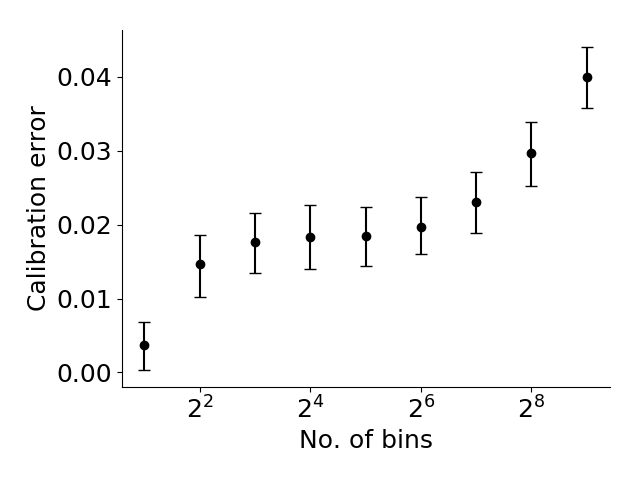
\includegraphics[width=\textwidth]{l2_lower_bound_imagenet_plot}
         \caption{ImageNet.}
         \label{fig:imagenet_lower_bound}
     \end{subfigure}
     \hfill
     \begin{subfigure}[b]{0.4\textwidth}
         \centering
         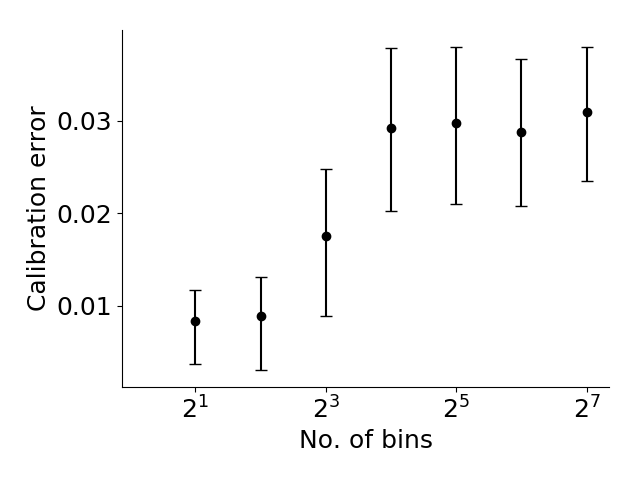
\includegraphics[width=\textwidth]{l2_lower_bound_cifar_plot}
         \caption{CIFAR-10.}
         \label{fig:cifar_10_lower_bound}
     \end{subfigure}
        \caption{
        Binned $\ell_2$ calibration errors of a recalibrated VGG-net model on CIFAR-10 and ImageNet with $90\%$ confidence intervals. The binned calibration error increases as we increase the number of bins. This suggests that binning cannot be reliably used to measure the true calibration error.
        }
        \label{fig:lower_bounds}
\end{figure}


% We might also wish to compare the calibration of different candidate models.

% \footnote{One possibility is to modify the calibration metric, for example to only require our model to be calibrated for all possible intervals of width $\geq \epsilon$.}

% One possibility is to modify the calibration metric, for example to only require our model to be calibrated for all possible intervals of width $\geq \epsilon$. 
% % This makes it difficult to ascertain if a model has a desired calibration error, or which of two models is better calibrated.

% We see three potential ways to resolve this:
% \begin{enumerate}
% \item Add a smoothness constraint on $E[Y | f(X)$], for example assume $E[Y | f(X)]$ is $L$-Lipschitz. Smoothness assumptions are common when training a model, but it is unsatisfying to assume a value of $L$, which we do not know, when \emph{evaluating} a model.
% \item Explore alternative metrics for calibration. For example, perhaps we only require our model to be calibrated for all possible intervals of width $\geq \epsilon$. 
% \item Discretize the outputs of the final model, so that it only outputs a finite number of values.
% \end{enumerate}

% In this paper we explore (3), but (1) and (2) are good directions for future research.



\section{The variance-reduced calibrator}
\label{sec:calibrating_models}

In the previous section we saw that the problem with scaling methods is we cannot estimate their calibration error. The upside of scaling methods is that if the function family is well suited to the data they require $O(1/\epsilon^2)$ samples to reach calibration error $\epsilon$, while histogram binning requires $O(B/\epsilon^2)$ samples where $B$ can be large. Can we get a method that is sample efficient to calibrate and one where it's possible to estimate the calibration error? To achieve this we propose the variance-reduced calibrator (Figure~\ref{fig:var_red_binning}) where we first fit a scaling function, and then bin the outputs of the scaling function. Note that in previous work binning the outputs of a function was used for evaluation, and without any guarantees, whereas in our case it is used for the method itself.

\subsection{Variance-reduced recalibration algorithm}

We split the recalibration data $T$ of size $n$ into 3 sets: $T_1$, $T_2$, $T_3$. The variance-reduced recalibration algorithm, illustrated in Figure~\ref{fig:variance_reduced_illustration}, outputs $\hat{g_{\mathcal{B}}}$ such that $\hat{g_{\mathcal{B}}} \circ f$ has low calibration error:

\textbf{Step 1 (Function fitting):} The first step is to select $g = \argmax_{g \in G} \sum_{(z, y) \in T_1} (y - g(z))^2$.
\pl{this should have been defined when you introduce Platt scaling}

\textbf{Step 2 (Bin construction):} The second step is to construct a suitable binning scheme. We choose the bins so that an equal number of $g(z_i)$ in $T_2$ land in each bin $I_j$ for each $j \in \{1, \dots, B\}$.

\textbf{Step 3 (Discretization):} The third step is to discretize $g$, by outputting the average $g$ value in each bin. Let $\mu(S) = \frac{1}{|S|} \sum_{s \in S} s$ denote the mean of a set of values.
Let $\hat{\mu}[j] = \mu(\{ g(z_i) \; | \; g(z_i) \in I_j \wedge (z_i, y_i) \in T_3 \})$ be the mean of the $g(z_i)$ values that landed in the $j$-th bin.
Then we set $\hat{g_{\mathcal{B}}}(z) = \hat{\mu}[\beta(g(z))]$ -- that is we simply output the mean value in the bin that $g(z)$ falls in.

\pl{this is the key part of your method; generally, I'd try to move as much out that's not new to existing work and highlight what's new in what you're doing}


\subsection{Analysis}

We show that the variance-reduced calibrator requires $O(B + 1/\epsilon^2)$ samples to calibrate, and in the next section we show that we can efficiently measure its calibration error. For the main theorem, we make some standard regularity assumptions on $\mathcal{G}$ (Lipschitz, injectivity, bounded parameters) which we formalize in Appendix~\ref{sec:calibrating_models_appendix}. These hold for Platt scaling, Beta calibration~\cite{kull2017sigmoids}, and vector scaling. Our result is a generalization result---we show that if $\mathcal{G}$ contains $g^*$ with low calibration error, then our method will quickly find $\hat{g}_{\mathcal{B}}$ with low calibration error:

\begin{restatable}[Calibration bound]{theorem}{finalCalib}
\label{thm:final-calib}
Suppose that $\min_{g \in \mathcal{G}}\ell_2^2\mbox{-CE}(g) \leq \epsilon^2$.
  Ignoring $\log$ factors, with $n = O(B + \frac{d'}{\epsilon^2})$ samples the variance-reduced calibration algorithm finds $\hat{g}_{\mathcal{B}}$ with $\ell_2^2\mbox{-CE}(\hat{g}_{\mathcal{B}}) \leq 2 \epsilon^2$. Note that $d'$ is the number of parameters which is $1$ for Platt scaling.
\end{restatable}

We present a proof in Appendix~\ref{sec:calibrating_models_appendix} but give a sketch here. Step 1 of our algorithm, essentially Platt scaling, simply fits a function $g$ to the data---standard statistical learning theory results show that $g$ converges in $O(\frac{1}{\epsilon^2})$ samples.

Step 3, where we bin the outputs of $g$, is the main variance-reduction step. If we had infinite data, Proposition~\ref{prop:bin_low_bound} showed that the binned version $g_{\bins{}}$ has lower calibration error than $g$, so we would be done. However we do not have infinite data---the core of our proof is to show that the empirically binned $\hat{g_{\bins{}}}$ converges to $g_{\bins{}}$ in $O(B + \frac{1}{\epsilon^2})$ samples, instead of $O(B + \frac{B}{\epsilon^2})$ samples in histogram binning. The intuition is in Figure~\ref{fig:variance_reduced_illustration}---the $g(z_i)$ values in each bin are in a narrower range than the $y_i$ values so when we take the average we incur less of an estimation error. The perhaps surprising part is that this leads to a provably smaller dependency on the number of bins $B$. In fact, there may be a small number of bins where the $g(z_i)$ values are not in a narrow range, but our proof still shows that the overall estimation error is small.

Recall that we were interested not only in producing a calibrated model, but one whose calibration error is measurable. Step 2, the bin construction step, plays a critical role here. We chose our bins so that each bin had an equal proportion of points---in order to estimate calibration error efficiently (Theorem~\ref{thm:final-ours}), we will require that this property approximately holds in the population as well.

\begin{definition}[Well-balanced binning]
Given a binning scheme $\mathcal{B}$ of size $B$, and $\alpha \leq 1$. We say $\mathcal{B}$ is $\alpha$-well-balanced if for all $j$,
\[ \frac{1}{\alpha B} \leq P(Z \in I_j) \leq \frac{\alpha}{B}\]
\end{definition}

\begin{lemma}
If $n \geq B\log{\frac{1}{\delta}}$, with probability at least $1 - \delta$, the binning scheme $\mathcal{B}$ we chose is 2-well-balanced.
\end{lemma}

While the way we choose bins is not novel, we believe the guarantees around it are. Not all binning schemes in the literature allow us to efficiently estimate the calibration error, for example the binning scheme in~\cite{guo2017calibration} does not. Our proof of this result, in the Appendix, uses a localized VC dimension argument. The core challenge here is that applying Chernoff bounds or a standardized VC dimension argument gives us a loose bound and tells us we need $O(B^2\log{\frac{1}{\delta}})$ samples which can be a bottleneck.

In Theorem~\ref{thm:sharpness-bound} in Appendix~\ref{sec:calibrating_models_appendix}, we also show that if we use lots of bins, discretization has little impact on model quality as measured by the mean-squared error.


\pl{I didn't find this section that satisfying;
first we should move stuff about scaling and binning out of this section and start this section by saying can we combine the best of the two worlds and mention $O(B + 1/\epsilon^2)$ - this is easy;
Then the big thing that's missing is the insight into why the proposed algorithm works and how the analysis proceeds,
kind of like a proof sketch
}

\subsection{Experiments}

Our experiments on CIFAR-10 and ImageNet show that in the low-data regime, for example when we use $\leq 1000$ data points to recalibrate, our variance-reduced calibration method produces models with much lower calibration error than histogram binning. The model's objective was to output a confidence score associated with each class, where we calibrated each class separately as in~\cite{zadrozny2002transforming}, used $B$ bins per class and evaluated calibration using the marginal calibration error (Definition~\ref{dfn:marginal-ce}).

We describe our experimental protocol for CIFAR-10.
The CIFAR-10 validation set has 10,000 data points. We sampled, with replacement, a recalibration set of 1,000 points. We ran either the variance-reduced calibrator (we fit a sigmoid in the function fitting step) or histogram binning and measured the marginal calibration error on the entire set of 10K points.
% \footnote{This is equivalent to using the empirical distribution on the 10K validation points as the true data distribution, and comparing how these methods perform. We do this since we cannot measure the ground truth calibration error.}
We repeated this entire procedure 100 times and computed mean and 90\% confidence intervals, and we repeated this varying the number of bins $B$. Figure~\ref{fig:marginal_calibrator_comparison_cifar} shows that the variance reduced calibrator produces models with lower calibration error, for example $35\%$ lower calibration error when we use 100 bins per class.

Using more bins allows a model to produce more fine-grained predictions e.g. (cite) use $B = 51$ bins. This improves the quality of predictions which can be measured by the mean-squared error -- Figure~\ref{fig:cifar_calibrator_cmp_mse_ce} shows that our method achieves better mean-squared errors for any given calibration constraint. More concretely, the figure shows a scatter plot of the mean-squared error and $\ell_2^2$ calibration error for histogram binning and variance-reduced calibration when we vary the number of bins. For example, if we want our models to have an $\ell_2^2$ calibration error $\leq 0.0004$ (which translates to an $\ell_2$ `average' calibration error of 2\%) we get a $10\%$ better mean-squared error. In the Appendix we give more experiment details and we show that these results hold for top-label calibration and for ImageNet.
% We also run an ablation to show that if we have more data points then as the theory predicts histogram binning catches up to the variance-reduced calibrator, and that the way we construct bins is crucial, the result do not hold if we use the binning scheme in~\cite{guo2017calibration}.

\begin{figure}
  \centering
  \centering
     \begin{subfigure}[b]{0.55\textwidth}
         \centering
         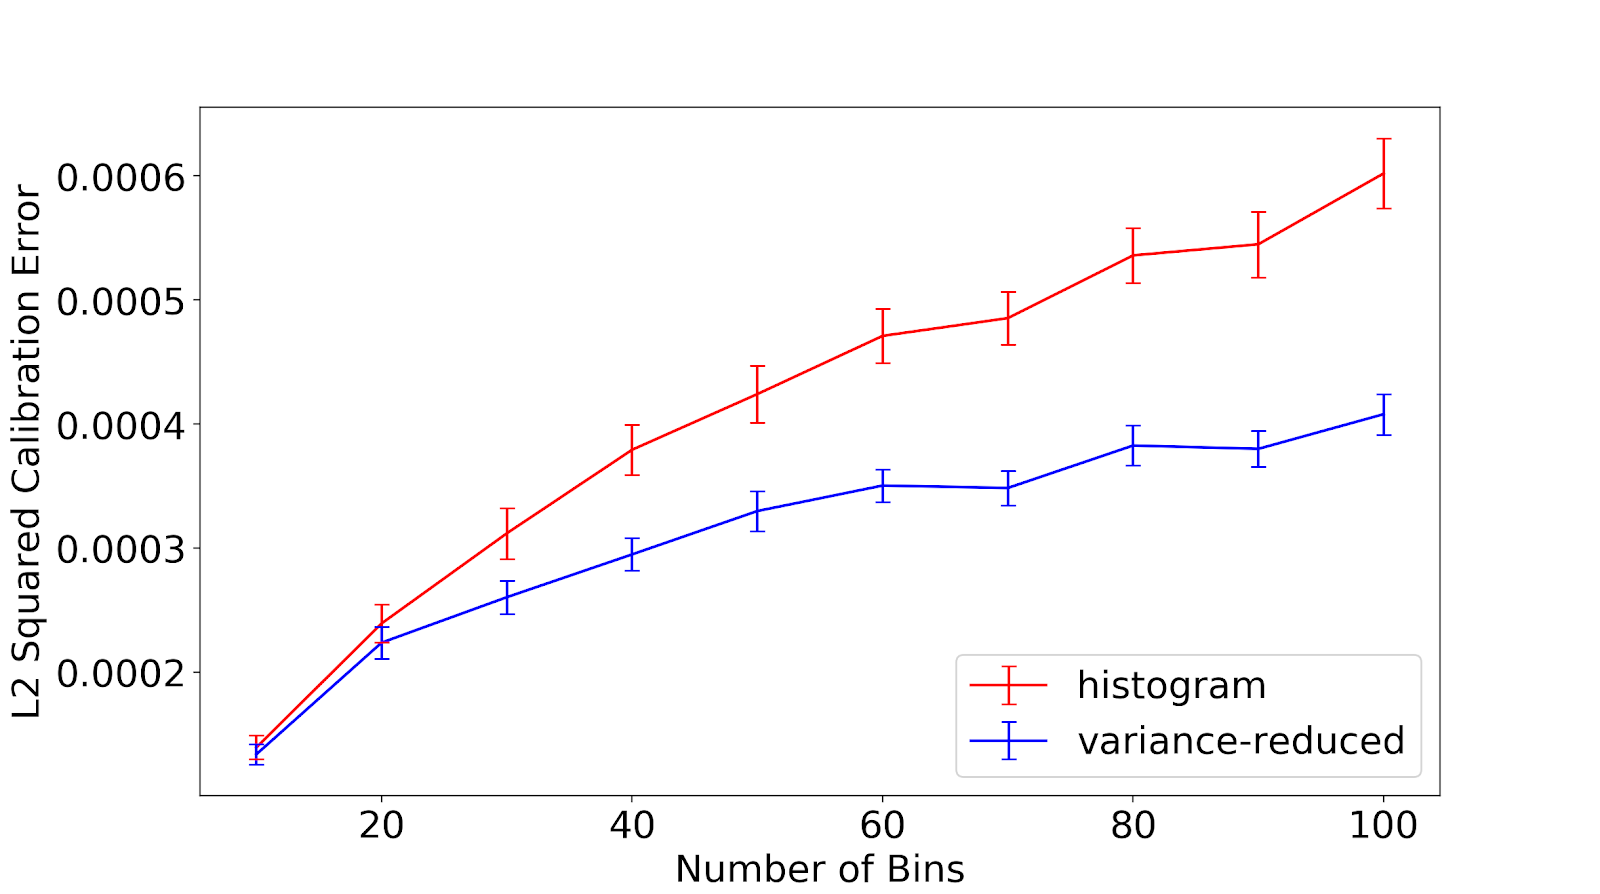
\includegraphics[width=\textwidth]{marginal_cifar_hist_vs_ours_bins.png}
         \caption{$\ell_2^2$ calibration error vs $B$.}
         \label{fig:marginal_calibrator_comparison_cifar}
     \end{subfigure}
     \hfill
     \begin{subfigure}[b]{0.4\textwidth}
         \centering
         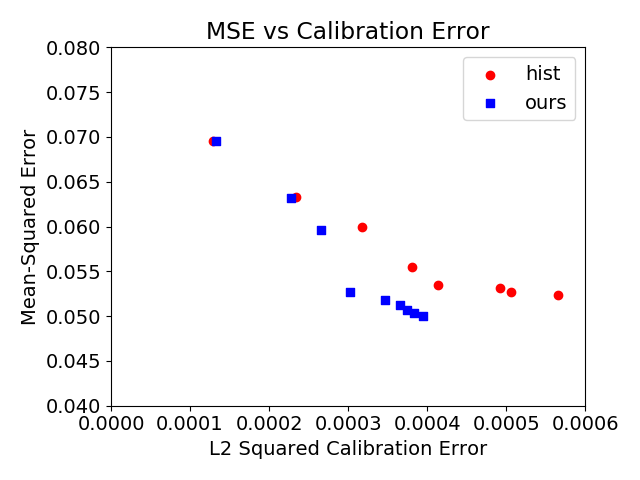
\includegraphics[width=\textwidth]{mse_vs_ce_calibrators_cifar.png}
         \caption{MSE vs $\ell_2^2$ calibration error.}
         \label{fig:cifar_calibrator_cmp_mse_ce}
     \end{subfigure}
  \caption{
  (\textbf{Left}) Recalibrating using 1,000 data points on CIFAR-10, our variance-reduced calibrator achieves lower $\ell_2^2$ calibration error than histogram binning, especially when the number of bins $B$ is large.
  (\textbf{Right}) For a fixed calibration error, our variance-reduced calibrator allows us to use more bins. This results in models with more predictive power which can be measured by the mean-squared error. Note the Y-axis range is $[0.4, 0.8]$ to zoom into the relevant region.
  }
  \label{fig:nan2}
\end{figure}



% Our experiments suggest that the binned calibration error gives us a poor sense of a model's calibration error if the model outputs a continuous range of values.
% We now turn to the question of how to produce models that we can \emph{verify} are calibrated.
% We describe \pl{propose} the \pl{the 'the' is bothering me a bit now that I keep on seeing it; strikes me as a bit presumptuous
% because it's like you're implicitly claiming that your estimator is the only one that reduces variance} variance-reduced calibrator (Figure~\ref{fig:variance_reduced_illustration}), and prove bounds on its sample complexity.
% In particular, assuming the function family $\mathcal{G}$ \pl{where did $\mathcal{G}$ come from? came out of nowhere} is well suited to recalibrate the data, we require $O(\frac{1}{\epsilon^2})$ samples to achieve calibration error $\epsilon$, while histogram binning requires $O(\frac{B}{\epsilon^2})$ samples.
% Moreover, unlike methods such as Platt scaling and temperature scaling, we can then check if our model is calibrated (see Section~\ref{sec:verifying_calibration}).
% If the model is not calibrated we can, for example, try different families $\mathcal{G}$ or collect more data and use histogram binning.
% \pl{I feel like this is getting too confusing;
% I'd just keep the story simple:
% begin by summarizing, in the previous section, we saw scaling techniques which are great because they are parametric, requiring only $O(1/\epsilon^2)$ to calibrate
% (explain because there's only one parameter (note that we didn't even explain Platt scaling, so this might be opaque),
% but the problem is that we can't estimate calibration error; On the other hand, we have histogram binning, which ... 
% Can we get something that's sample efficient to calibrate and one where it's possible to estimate the calibration error?
% this is the heart of this paper, so need to spell it out slowly;
% here is the time to use Figure 1 too explain your method
% }

% Models obtained by performing empirical risk minimization on a training set tend to be uncalibrated. Typically, we apply recalibration methods that take the output of an uncalibrated model, and transform it into a calibrated probability. These methods require additional held-out \emph{recalibration data}. 

% \textbf{Recalibration framework:} We now turn to the question of how to produce models that \emph{we can verify are calibrated}. Models obtained by performing empirical risk minimization on a training set tend to be uncalibrated. Typically, we apply post-processing methods that take the output of an uncalibrated model, and transform it into a calibrated probability. These methods require an additional held-out \emph{calibration set}.

% \textbf{Histogram binning:} One common method for recalibration is histogram binning. The outputs of the model (on the calibration set) are divided into disjoint intervals $I_1, ..., I_B$. At test time, if the model's output falls into interval $I_j$, we output $s_j$ where $s_j$ is the proportion of examples in $I_j$ that were positive in the calibration set. \ak{Either make more clear and/or refer to another paper} The advantage of histogram binning is that in the limit of infinite data it will be perfectly calibrated. However, achieving $\ell_2$ calibration error $\epsilon$ with $B$ bins can require up to $O(\frac{B}{\epsilon^2})$ samples.

% \textbf{Variance-reduced calibration:} We introduce variance-reduced calibration, a more sample-efficient way to calibrate, and analyze the sample complexity of our methods. Like in Platt scaling, we first fit a function from a function family $\mathcal{F}$ to the data. Then, we identify a suitable binning scheme, and discretize the outputs of our model. Restricting to the function family $\mathcal{F}$ introduces some bias -- if $\mathcal{F}$ is poorly chosen, then even in the limit of infinite data we may not be able to calibrate. However, if $\mathcal{F}$ is well-chosen, we will be able to calibrate with far fewer samples.

% \textbf{Calibration verifiable:} Moreover, unlike methods such as Platt scaling and temperature scaling, we can then check if our model is calibrated using techniques described in the previous section. If the model is not calibrated we can, for example, try different families $\mathcal{F}$ or collect more data and use histogram binning.

% The highlights of our analysis include:
% \begin{enumerate}
% \item We show that discretizing approaches like Platt scaling, isotonic regression, or temperature scaling, requires very few samples (Theorem~\ref{thm:empirical-binning}). Surprisingly, the number of samples required only has logarithmic dependencies on $B$.
% \item We show that we only need $n = O(B\log{B})$ samples to select a lower-balanced binning scheme (Theorem~\ref{thm:well-ba-binning}). Standard results on concentration of functions like Dvoretzky–Kiefer–Wolfowitz or VC dimension give us $n = O(B^2\log{B})$.
% \item We show that discretizing the outputs of our model has little impact on model quality, measured in terms of the Brier score (also known as the mean-squared error) (Theorem~\ref{thm:sharpness-bound}).
% \end{enumerate}
% We believe we are the first to give a formal framework for the statistics of calibration, which can guide future work in this area.

% There are two general approaches to recalibration. The first is histogram binning, where we output the average label value observed in each bin. The advantage of histogram binning is that in the limit of infinite data it will be perfectly calibrated. However, to achieve $\ell_2$ calibration error $\epsilon$ with $B$ bins it requires $O(\frac{B}{\epsilon^2})$ samples.\footnote{This analysis is standard, so we omit it from our paper.} The second is to fit a function, like a sigmoid function in the case of Platt scaling, and then discretize the model outputs. If this approach can calibrate to within error $\epsilon$,\footnote{Depending on the function family, this approach may, or may not, ever achieve good calibration.} it requires only $O(\frac{1}{\epsilon^2})$ samples to do so. In particular, estimating the calibration error ($O(\frac{B}{\epsilon^2})$ with prior approaches, and $O(\frac{\sqrt{B}}{\epsilon^2})$ with our estimator) is then the bottleneck. This is the focus of our analysis which concludes with Theorem~\ref{thm:final-calib} and Theorem~\ref{thm:sharpness-bound}. In practice, we would try multiple re-calibration approaches, estimate the calibration error using our estimator, and choose the best one.

% Suppose we are given a trained model $f: \mathcal{X} \to \mathcal{Z}$ that we wish to calibrate. As before, $X \in \mathcal{X}$ and $Y \in \{0, 1\}$ are random variables denoting the input and label, given by an unknown joint distribution $P(X, Y)$. \pl{don't need to repeat again} We wish to learn $\hat{g_{\mathcal{B}}} : \mathcal{Z} \to [0, 1]$ such that $\hat{g_{\mathcal{B}}} \circ f$ is well-calibrated. \pl{if you want this, this should have gone in the setup} Let $Z = f(X)$.

% Let $\mathcal{G}$ be a family of functions from $\mathcal{Z} \to [0, 1]$, and $B$ be the number of outputs \pl{don't like this terminology} for the final model. Like other calibration methods, we require additional i.i.d. calibration data $T = \{ z_i, y_i \}_{i=1}^n$ where $z_i, y_i \sim P(Z, Y)$ for all $i$. We split $T$ into 3 sets: $T_1$, $T_2$, $T_3$. We begin with a definition.

% \begin{definition}[Binning schemes]
% A binning scheme $\mathcal{B}$ of size $B$ is a set of $B$ intervals $I_1, \dots, I_j$ that partitions $[0, 1]$. Given an input $x \in [0, 1]$ we might want to know what bin it falls in -- if $x \in I_j$ let $\beta(x) = j$.
% % into $B$ disjoint intervals or bins, defined by bin boundaries $0 = b_0 < b_1 < ... < b_B = 1$. For $1 \leq j \leq B$, the $j$-th bin is the interval $I_j$ where $I_1 = [b_0, b_1]$ and $I_j = (b_{j-1}, b_j]$ for $j > 1$. 
% \end{definition}

% \footnote{The optimal way to select $T$ depends on $F$, and our analysis in the next subsection.}

% Formally, given interval $I$ and dataset $T$, let $N(I, T) = \frac{1}{|T|}\sum_{(z, y) \in T} \mathbb{I}(g(z) \in I)$. We choose bins such that \pl{English first} $N(I_j, T_2) = \frac{1}{B}$ for all $1 \leq j \leq B$. 
% \pl{I think you should move this out to a separate section on histogram binning}

% Let $R_j(T) = \{ g(z_i) \; | \; g(z_i) \in I_j \wedge (z_i, y_i) \in T \}$.
% Let $\hat{\mu}[j] = \mu(R_j(T_3))$ be the mean of the $g(z_i)$ values in the $j$-th bin.


% \begin{restatable}[Calibration bound]{theorem}{finalCalib}
% \label{thm:final-calib}
% Suppose that $\min_{g \in \mathcal{G}}\ell_2^2\mbox{-CE}(g) \leq \epsilon^2$.
%   Ignoring $\log$ factors, with $n = O(B + \frac{L^2 (d')^2}{\epsilon^2})$ \pl{$L^2$ not defined} samples the variance-reduced calibration algorithm produces a 2-well-balanced binning scheme and $\hat{g}_{\mathcal{B}}$ with $\ell_2^2\mbox{-CE}(\hat{f}_{\mathcal{B}}) \leq 2 \epsilon^2$. Note that $d' = 1$ for Platt scaling.
% \end{restatable}


 % The key steps are to (1) show that by optimizing the mean-squared error we will find a $g \in \mathcal{G}$ with low calibration error, (2) the binning scheme we constructed is 2-well-balanced (on the population), and finally (3) the number of samples required to empirically discretize $g$ to get $\hat{g}_{\mathcal{B}}$ only has logarithmic dependencies on the number of outputs $B$.

% Our analysis \pl{what are we analyzing?} requires some assumptions on the function family $\mathcal{G}$:
% \begin{enumerate}
% \item (Finite bounded parameters). Let $\mathcal{G} = \{ g_{\theta} : \mathcal{Z} \to [0, 1] \; | \; \theta \in \mathbb{R}^{d'} \wedge ||\theta||_{\infty} \leq B \}$
% \item (Injective). For all $g_{\theta} \in \mathcal{G}$ we assume $g_{\theta}$ is injective.
% \item (Lipschitz). Suppose that for all $z$, $|g_{\theta_1}(z) - g_{\theta_2}(z)| \leq L|\theta_1 - \theta_2|_2$.
% \end{enumerate}

% Assumptions (1) and (3) are standard in statistical learning theory. Assumption (2) \pl{what about 1 and 3} holds for methods like Platt scaling, Beta calibration~\cite{kull2017sigmoids}, and vector scaling, but we hope future work relaxes this \pl{huh? why would you relax this if you just said it holds}.
% \pl{this paragraph is confusing - all you want to say is that these assumptions hold for X, Y, Z}

% \pl{Also, I feel like analyzing $\mathcal{G}$ is not the focus of this paper - this is really some orthogonal problem, right?
% it should just be obvious that in Platt scaling, you're just fitting a single parameter, your error's going to be low...
% we want to spend time talking about the discretization
% }




% We assume the function family $\mathcal{F}$ is chosen such that given infinite data, minimizing the mean-squared error loss leads to a well-calibrated solution.

% \begin{proposition}[Error from empirical risk minimization]
% \label{thm:mse-convergence}
%  There exists a constant $c$ such that the following holds. For $\theta \in  \mathbb{R}^{d'}$ let $f_{\theta} : \mathcal{Z} \to [0, 1]$ be injective. Suppose that for all $z$, $|f(z; \theta_1) - f(z; \theta_2)| \leq L|\theta_1 - \theta_2|_2$. Let $\mathcal{F} = \{ f_{\theta} \; | \; \theta \in \mathbb{R}^{d'} \wedge ||\theta||_{\infty} \leq B \}$, and let $f^* = \argmin_{f \in \mathcal{F}}{E[(f(Z) - Y)^2]}$. Then with probability $\geq 1 - \delta$ (over the samples) $\ell_2\mbox{-CE}(f) \leq \ell_2\mbox{-CE}(f^*) + \frac{cLd' \log{B/\delta}}{\sqrt{n}}$. 
% \end{proposition}

% We chose a binning scheme such that each bin had an equal proportion of points in the calibration set. We show that this property approximately holds in the population as well.

% \begin{definition}[Well-balanced binning]
% Given a binning scheme $\mathcal{B}$ of size $B$, and $\alpha \leq 1$. We say $\mathcal{B}$ is $\alpha$-well-balanced if for all $j$,
% \[ \frac{1}{\alpha B} \leq P(Z \in I_j) \leq \frac{\alpha}{B}\]
% \end{definition}

% \begin{theorem}[Population well-balanced]
% \label{thm:well-ba-binning}
% If we use $O(B \log{B})$ samples in step 2 of our algorithm, the binning scheme we select will be 2-well-balanced.
% \end{theorem}

% Next, we show that if we had infinite data, discretizing $f$ can only decrease its calibration error.

% \begin{definition}
% Given $f : \mathcal{Z} \to [0, 1]$, and a binning scheme $\mathcal{B}$, let $f_{\mathcal{B}}$ denote the discretized version of $f$ where we take the average value of $f$ in each bin. Formally, $f_{\mathcal{B}}(z) = \mathbb{E}[f(Z) | f(Z) \in I_{\beta(f(z))}]$. 
% \end{definition}

% \begin{lemma}[Binning improves calibration]
% \label{lem:inf-binning}
% [Binning improves calibration] Given $f : \mathcal{Z} \to [0, 1]$ and binning scheme $\mathcal{B}$, $\ell_2\mbox{-CE}(f_{\mathcal{B}}) \leq \ell_2\mbox{-CE}(f)$.
% \end{lemma}

% In step 3 of our algorithm, we use finitely many samples to discretize the outputs of $f$, to get an approximation $\hat{f_{\mathcal{B}}}$. We show that $f_{\mathcal{B}}$ -- the discretized version of $f$ when we have infinite data -- and $\hat{f_{\mathcal{B}}}$ are close in both $\ell_1$ and $\ell_2$ distance.

% \begin{definition} [$\ell_1, \ell_2$ distance]
% Given $f, g : \mathcal{Z} \to [0, 1]$, we define $|f - g|_2^2 = \mathbb{E}[(f(Z) - g(Z))^2]$, $||f- g||_2 = \sqrt{|f - g|_2^2}$, and $|f- g|_1 = \mathbb{E}[\lvert f(Z) - g(Z) \rvert]$.
% \end{definition}

% \begin{theorem}[Error from empirical binning]
% \label{thm:empirical-binning}
% There exist constants $c_B, c_1, c_2$ such that the following is true. Given $f : \mathcal{Z} \to [0, 1]$, binning set $T = \{(z_i, y_i)\}_{i=1}^n$ and a 2-well-balanced binning scheme $\mathcal{B}$ of size $B$. Given $0 < \delta < 0.5$, suppose that $n \geq c_B B\log{\frac{B}{\delta}}$. Then with probability at least $1 - \delta$,  $|\hat{f_{\mathcal{B}}} - f_{\mathcal{B}}|_2 \leq \frac{c_2}{\sqrt{n}}\sqrt{\log{\frac{B}{\delta}}}$ and $|\hat{f_{\mathcal{B}}} - f_{\mathcal{B}}|_1 \leq \frac{c_1}{\sqrt{nB}}\sqrt{\log{\frac{B}{\delta}}}$
% \end{theorem}

% We use this to bound the calibration error of $\hat{f_{\mathcal{B}}}$ with a simple lemma.

% \begin{lemma}
% For all $f, g : Z \to [0, 1]$, $\ell_2\mbox{-CE}(f) \leq \ell_2\mbox{-CE}(g) + |f - g|_2$.
% \end{lemma}

% Putting these together, we get our final bound on calibration error.

% Further\pl{more}, the binning scheme $\mathcal{B}$ we produce will be 2-well-balanced, which will allow us to measure the calibration error efficiently, as described in the next section (Theorem~\ref{thm:final-ours}).



% We give a proof of this result in the Appendix. The key steps are to (1) show that by optimizing the mean-squared error we will find a $g \in \mathcal{G}$ with low calibration error, (2) the binning scheme we constructed is 2-well-balanced (on the population), and finally (3) the number of samples required to empirically discretize $g$ to get $\hat{g}_{\mathcal{B}}$ only has logarithmic dependencies on the number of outputs $B$.

% We also show that if we use lots of bins, discretization has little impact on model quality as measured by the Brier score (the mean-squared error):

% \pl{we never mentioned sharpness and MSE is not sharpness}
% \begin{theorem}[Sharpness bound]
% \label{thm:sharpness-bound}
% If $\mathcal{B}$ is a 2-well-balanced binning scheme of size $B$ and $B \leq O(n\log{n})$, then with high probability $\mbox{MSE}(\hat{g}_{\mathcal{B}}) \leq \mbox{MSE}(g) + O(\frac{1}{B})$.
% \end{theorem}


\section{Verifying calibration}
\label{sec:verifying_calibration}

\newcommand{\pluginEst}[0]{\ensuremath{\hat{E}_{pl}^2}}
\newcommand{\cancelEst}[0]{\ensuremath{\hat{E}^2}}
\newcommand{\ltwoerror}[0]{\ensuremath{{\hat{E}^*}^2}}
\newcommand{\piSmallBound}[0]{\ensuremath{\frac{12}{n}\log{\frac{2B}{\delta}}}}

\pl{isn't a easier way of saying this, we can only estimate the calibration error of binned calibrators? as we showed in previous section}
If a model outputs values from some finite set $S$,\footnote{The model can choose the set $S$.} and the probability of outputting each value $s \in S$ is not too small, then we can estimate its calibration error. The plugin estimator \pl{explain this (make simple things simple)} used in past work requires samples proportional to the number of model outputs $|S|$. Instead, we introduce the \emph{cancelling} estimator that requires samples proportional to $\sqrt{|S|}$. At a high level, the cancelling estimator leverages cancellation of error terms across different bins.

\pl{why not use $B$ instead of $|S|$?}
\pl{I guess there's a subtlety that here, we're talking about specific values not bins...}

% We prove these finite sample guarantees (Theorem~\ref{thm:final-ours}), and show experimental evidence that our estimators approximate the calibration error better. We also show, experimentally, that using a better estimator allows us to pick out better models.

The plugin estimator directly estimates each term in the $\ell_2^2$ calibration error from samples~\cite{nguyen2015posterior, hendrycks2019anomaly, kuleshov2015calibrated, hendrycks2019pretraining}. Suppose we wish to measure the calibration error of a model $f : \mathcal{X} \to S$ where $S \subseteq [0, 1]$. Order the elements in $S$: $s_1 < s_2 < \dots < s_B$, where $B = |S|$ denotes the number of model outputs. Suppose we get an evaluation set $T_n = \{(x_1, y_1), \dots, (x_n, y_n)\}$ sampled i.i.d. from $P(X, Y)$.

\pl{notationally, you can index directly using $s$ instead of $i$ to save one level of indirection}

\begin{restatable}[Plugin estimator]{definition}{pluginDfn}
\label{dfn:plugin-estimator}
\pl{English: define $\hat y_i$ to be the empirical average for the $i$-th score}
  Let $L_i = \{ y_j \; | \; (x_j, y_j) \in T_n\wedge f(x_j) = s_i \}$ \pl{background this} denote the label values where the model outputs $s_i$.

We estimate $E[Y | f(X) = s_i]$ as:
\[ \hat{y_i} = \sum_{y \in L_i} \frac{y}{|L_i|} \] 
  \pl{English: define $\hat p_i$ to be the actual average for the $i$-th score}
We estimate $P(f(X) = s_i)$ by:
\[ \hat{p_i} = \frac{|L_i|}{n} \]
  Then the plugin estimator for the $\ell_2^2$ error is \pl{the weighted squared difference between the two}:
  \pl{$b$ should be upper case (see throughout)}
  \pl{but if you use the notation, then you have
  \[ \mathcal{E}_\text{plugin} = \sum_{s \in S} \hat{p_s} (s - \hat{y_s})^2 \]
  }
\[ \pluginEst{} = \sum_{i=1}^B \hat{p_i} (s_i - \hat{y_i})^2 \]
\end{restatable}
\pl{can we just use $L^2$ for this whole paper?}

We now define our improved cancelling estimator. The key insight is that the plugin estimate of the error in each bin, $(s_i - \hat{y_i})^2$ is biased. By debiasing these estimates we get cancellations across bins.

\pl{this formula is a bit out of nowhere; saying 'debiasing' is helpful, but can you actually say the criteria more formally and declaratively?}
\begin{restatable}[Cancelling estimator]{definition}{cancelingDfn}
The cancelling estimator for the $\ell_2^2$ error is:
\[ \hat{E}^2 = \sum_{i=1}^b \hat{p_i} \Big[ (s_i - \hat{y_i})^2 - \frac{\hat{y_i}(1 - \hat{y_i})}{\hat{p_i}n-1} \Big] \]
\end{restatable}

The main results are that to check if the $\ell_2^2$ calibration error of a model is $\leq \epsilon^2$, the plugin estimator requires $\Theta(\frac{B}{\epsilon^2})$ samples (Theorem~\ref{thm:final-plugin}) while our estimator requires $\theta(\frac{\sqrt{B}}{\epsilon^2})$ samples (Theorem~\ref{thm:final-ours}). We begin by giving a bound on the error of the plugin estimator.

\begin{restatable}{theorem}{pluginBound}
\label{thm:plugin-bound}
Let $p_i = P(f(X) = s_i)$ and suppose $p_i > \piSmallBound{}$ for all $i$. Let $c(n)$ be defined as:
\[ c(n) = \sqrt{\frac{3}{n \min p_i} \log{\frac{2B}{\delta}}} \]
Then for the plugin estimator, with probability at least $1 - 3\delta$,
\[ | \hat{E_{pl}}^2 - {E^*}^2 | \leq c(n){E^*}^2 + \sqrt{\frac{2(1+c(n)){E^*}^2}{n} \log{\frac{2}{\delta}}} + \frac{B}{2n} \log{\frac{2B}{\delta}} \]
\end{restatable}

Typically, we are interested in checking if our model has calibration error $\leq \epsilon$ \pl{but this is not what we actually show due to $r$}. \pl{say that the next theorem studies this} In other words, we are given $\epsilon, \delta > 0$ and effect size $0 < r < 1$ \pl{where did effect size come from? I think all of this should be set up as what we want before doing the analysis}. If the calibration error is $> \epsilon$, then with probability at least $1 - \delta$ we should output that it is not calibrated \pl{be more precise}. If the calibration error is $< r\epsilon$, then with probability at least $1 - \delta$, we should output that the model is calibrated.

\begin{restatable}[Plugin bound]{theorem}{finalPlugin}
\label{thm:final-plugin}
  Suppose \pl{use English} $\forall i.\;p_i \geq \frac{1}{2B}$ and $n = \Theta(\frac{B}{\epsilon^2})$ ignoring $\log$ factors. Then the plugin estimator can check if ${E^*}^2 \leq \epsilon^2$ with failure probability $\delta$, and constant effect size $0 < r < 1$. 
\end{restatable}

Another way of thinking about this is that if $n = \Theta(\frac{B}{{E^*}^2})$ then \pl{English} $r {E^*}^2 \leq \hat{E_{pl}}^2 \leq (1+r){E^*}^2$.

\pl{should be separate subsection}
Next we bound the error of the cancelling estimator.

% \subsection{Analysis of our estimator}

\begin{restatable}{theorem}{cancelingBound}
\label{thm:our-bound}
Let $p_i = P(f(X) = s_i)$ and suppose $p_i > \piSmallBound{}$ for all $i$. Let $c(n)$ be as defined in Theorem~\ref{thm:plugin-bound}.
Then for the cancelling estimator, with probability at least $1 - 4\delta$,
\[ | \hat{E}^2 - {E^*}^2 | \leq c(n){E^*}^2 + \sqrt{\frac{2(1+c(n)){E^*}^2}{n} \log{\frac{2}{\delta}}} + \frac{3\sqrt{B}}{n} \log{\frac{n}{\delta}} + \frac{\delta}{n}\]
\end{restatable}


\begin{restatable}[Cancelling bound]{theorem}{finalCanceling}
\label{thm:final-ours}
Suppose $\forall i.\;p_i \geq \frac{1}{2B}$ and $n = \Theta(B+\frac{\sqrt{B}}{\epsilon^2})$ ignoring $\log$ factors. Then the cancelling estimator can check if ${E^*}^2 \leq \epsilon^2$ with failure probability $\delta$ and constant effect size $r$. 
\end{restatable}
\tm{may be good to explain what's the dominating term. How to interpret the bound ---}
\pl{provide a few sentences for proof sketch - at least the highlights - standard concentration or anything new? what's the hard part?}

\subsection{Experiments}

We ran experiments on CIFAR-10 and Imagenet to compare the practical performance of the cancelling estimator and the plugin estimator. We split the validation set \pl{how big?} into two chunks $C_1$ \pl{maybe give these more meaningful names with subscripts? anyway, put them behind macros} and $C_2$ \pl{what sizes}. We use $C_1$ to re-calibrate and discretize a trained model using $B = 100$ bins. For varying values of $n$, we sample $n$ points, with replacement, from $C_2$, and estimate the calibration error using the cancelling estimator and the plugin estimator. We then compute the squared deviation of these estimates from the calibration error measured on the entire chunk $C_2$. We repeat this 1,000 times to get the mean squared deviation and confidence intervals. The results are in Figure~\ref{fig:mse_estimators}. \pl{always say what the result is: Figure shows that...}
In the Appendix, we include results for ImageNet, ablations on $B$, and we visualize the histogram of the deviations.

\pl{say explicitly that we never say 'not calibrated'; there's a disconnect between the theory, which requires $r$ and $\epsilon$ and what we're doing here}

We also run a multi-class calibration experiment on CIFAR-10 to show that our estimator allows us to select models with a better \pl{lower} Brier \pl{should we just say MSE everywhere? just be consistent since you defined MSE at the beginning} score subject to a given calibration constraint. As before, we split the validation set into $C_1$ and $C_2$. On $C_2$, we estimate the calibration error using the plugin and cancelling estimators and use 100 Bootstrap resamples to compute a 90\% upper confidence bound on the estimate. We compute the Brier scores and the upper bounds on the calibration error for $B = 10, 15, \cdots, 100$ and show the Pareto curve in Figure~\ref{fig:mse_vs_ce_estimators}. The results show that for any desired calibration error, the cancelling estimator enables us to pick out models with a better Brier score.

\begin{figure}
  \centering
  \centering
     \begin{subfigure}[b]{0.45\textwidth}
         \centering
         \includegraphics[width=\textwidth]{mse_estimator_100_bins.png}
         \caption{Mean-squared errors of estimates.
         \pl{s/ours/canceling}
         \pl{Number of samples of what - relate to notation in text}
         \pl{label y-axis}
         }
         \label{fig:mse_estimators}
     \end{subfigure}
     \hfill
     \begin{subfigure}[b]{0.45\textwidth}
         \centering
         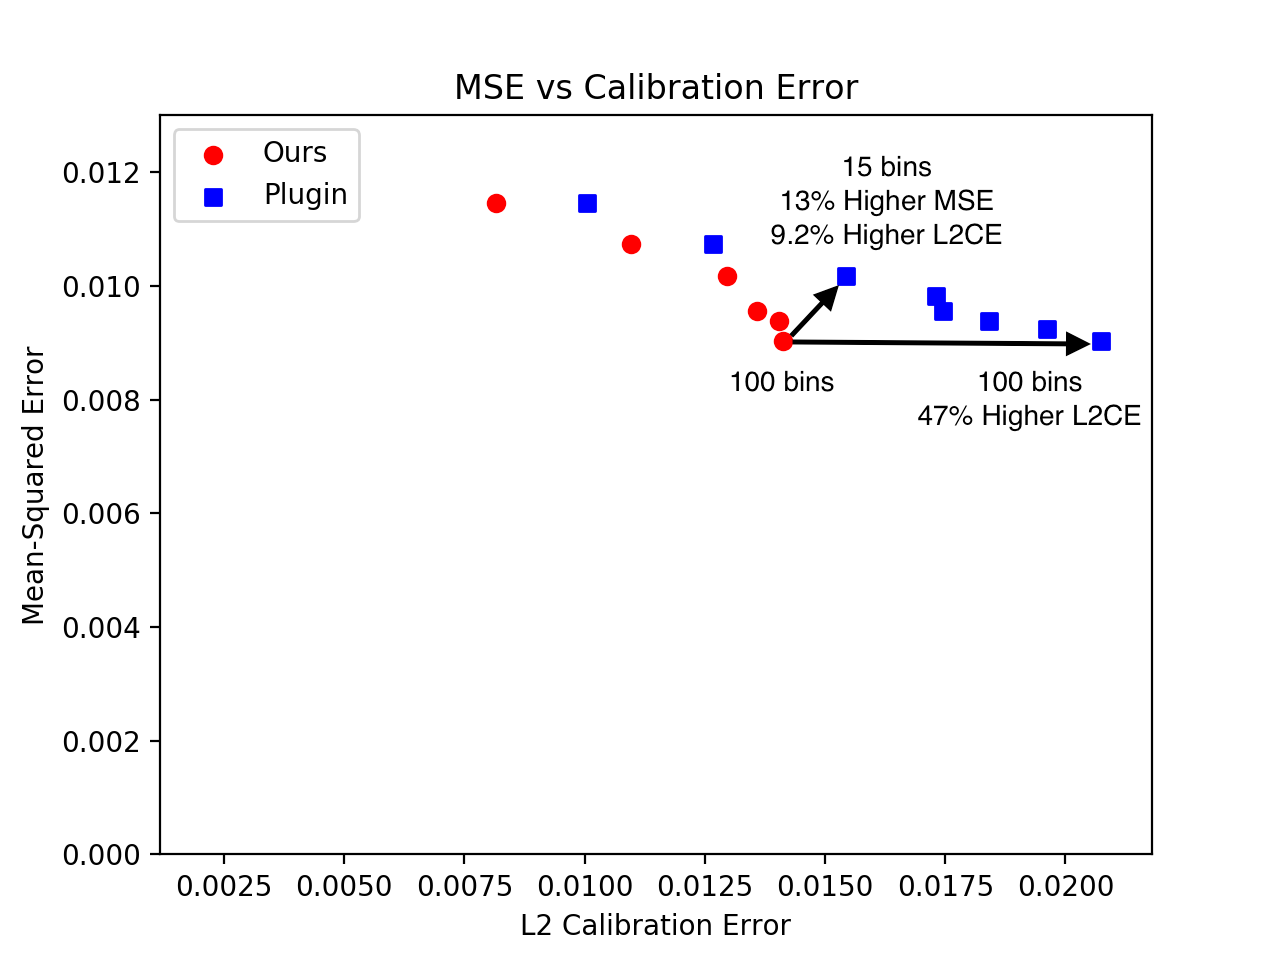
\includegraphics[width=\textwidth]{mse_vs_verified_error_plugin_vs_ours.png}
         \caption{Brier score vs calibration error.
         \pl{be consistent with MSE/Brier}
         \pl{make text larger by reducing the xrange and yrange}
         }
         \label{fig:mse_vs_ce_estimators}
     \end{subfigure}
  \caption{
    (\textbf{Left}) Mean-squared errors of cancelling and plugin estimators on a recalibrated VGG-net model on CIFAR-10 with $90\%$ confidence intervals (lower values better). Our estimator is closer to the ground truth \pl{what's ground truth? 0 on the y-axis?}.
  (\textbf{Right}) Plot of Brier scores against upper bounds \pl{90\% confidence bounds or something?} on the calibration error computed by our estimator and the plugin estimator, when we vary the number of bins $B$. For a given calibration error, our estimator enables us to choose models with a better Brier score. If we want a model with $\ell_2$ calibration error less than 0.015, the cancelling estimator tells us we can confidently use 100 bins, while relying on the plugin estimator only lets us use 15 bins and incurs a 13\% higher Brier score.
  \pl{I find it awkward that you have MSE (which is squared) plotted against calibration error (non-squared);
  can we just make it RMSE instead?
  }
}
  \label{fig:mse_estimators_bins}
\end{figure}

% This means that our estimator has a substantially better dependency on the number of outputs of the model.

% \begin{corollary}
% \label{cor:final-ours}
% Using our estimator $\hat{E}$, if $n = \Theta(kb + \frac{\sqrt{b}}{\epsilon^2})$ ignoring $\log$ factors, we can check if $|{E^*} | \leq \epsilon$ with significance and power $\delta$, and constant effect size $r$. 
% \end{corollary}


\section{Related work}

Calibration has been studied and used in many fields including meteorology~\cite{murphy1973vector, murphy1977reliability, degroot1983forecasters,gneiting2005weather, brocker2009decomposition}, medicine~\cite{jiang2012calibrating, crowson2017calibration, harrell1996prognostic}, reinforcement learning~\cite{malik2019calibrated}, natural language processing~\cite{nguyen2015posterior, card2018calibration}, speech recognition~\cite{dong2011calibration}, econometrics~\cite{gneiting2007probabilistic}, and psychology~\cite{lichtenstein1982calibration}. Our work is inspired in part by recent methods for calibration~\cite{guo2017calibration, kuleshov2018accurate, hendrycks2019anomaly}. In these papers, binning is used to evaluate the calibration error of models, whereas in our case it is part of the method itself, which is key to the guarantees we give. Besides the calibration error metric, prior work also uses the Hosmer-Lemeshov test~\cite{hosmer1980goodness} and reliability diagrams~\cite{degroot1983forecasters, brocker2007reliability} to evaluate calibration. Besides calibration, there are many other ways of producing and quantifying uncertainties, including Bayesian methods~\cite{gelman1995bayesian} and conformal prediction~\cite{shafer2008tutorial, lei2016distribution}.

Bias is a common issue with statistical estimators, for example for the sample standard deviation. It has also long been known that the mean-squared error, measured on samples, gives a biased estimate---the seminal work by Stein~\cite{stein81sure} investigates and fixes this bias. However, debiasing an estimator does not typically lead to \emph{an improved sample complexity.}

\pl{first impression is that this looks really brief...you can say calibration has been studied traditionally in many fields: meteorology (cite), ML (cite), etc.;
then is there's probably non calibration work that's related...just non-parametric function estimation...how is calibration different?
anything related for proof techniques?
}

\section{Conclusion}

In this paper we had three contributions: 1. We showed that the calibration error of popular continuous models is underestimated; 2. We introduced the first method, to our knowledge, that has better sample complexity than histogram binning but has a \emph{measurable calibration error}, giving us the best of both worlds of scaling and binning; and 3. We showed that an alternative estimator has better sample complexity than the commonly used plugin estimator. Our method gives us 35\% lower calibration error on CIFAR-10, and up to 5x lower calibration error on ImageNet, when we use $B = 100$ bins.

% We hope future work looks at even stronger notions of multiclass calibration (prior work typically focuses on top-label calibration) and calibration under domain shift.

% We think our framework opens up many new avenues for exploration. Can we come up with a binning scheme that is better than the well-balanced binning scheme that is one that leads estimate the calibration error even faster, at least for 

% \tm{I guess we need a conclusion section. }

% \tm{briefly summarize the contribution (now we can use slightly different language because we assume the readers have read most of the paper and now the definitions.)}
% \tm{Open question or future directions, potential implication of the paper}



\bibliographystyle{unsrtnat}
\bibliography{local,refdb/all}

\appendix

\newpage 
\section{Model and code details}

The VGG16 model we used for ImageNet experiments is from the Keras~\cite{chollet2015} module in the TensorFlow~\cite{tensorflow2015-whitepaper} library and we used pre-trained weights supplied by the library. The VGG16 model for CIFAR-10 was obtained from an open-source implementation on GitHub~\cite{geifman2017}, and we used the pre-trained weights there. We independently verified the accuracies of these models.

\pldel{We include our code for the experiments in the supplementary material.}

\newpage
\section{Ablations for Section~\ref{sec:challenges-measuring}}
\label{sec:appendix_platt_experiments}

Here we present additional experiments for Section~\ref{sec:challenges-measuring}.
Recall that the experiments in section~\ref{sec:challenges-measuring} showed that binning underestimates the calibration error of a model---we focused on the $\ell_2\mbox{-CE}$ and selected bins so that each bin has an equal number of data points. Figure~\ref{fig:imagenet_lower_bound_l1} shows that binning is also unreliable at measuring the $\ell_1\mbox{-CE}$ on ImageNet---using more bins uncovers a higher calibration error than we would otherwise detect with fewer bins. Figure~\ref{fig:imagenet_lower_bound_l1_prob} shows that the same conclusion holds on ImageNet if we look at the $\ell_1\mbox{-CE}$ \emph{and} use an alternative approach to selecting bins used in~\cite{guo2017calibration} that we call \emph{equal-probability binning}. Here, the $B$ bins are selected to be $I_1 = [0, \frac{1}{B}], I_2 = (\frac{1}{B}, \frac{2}{B}], \dots, I_B = (\frac{B-1}{B}, 1]$. The experimental protocol is the same as in section~\ref{sec:challenges-measuring}.

\begin{figure}
     \centering
     \begin{subfigure}[b]{0.45\textwidth}
         \centering
         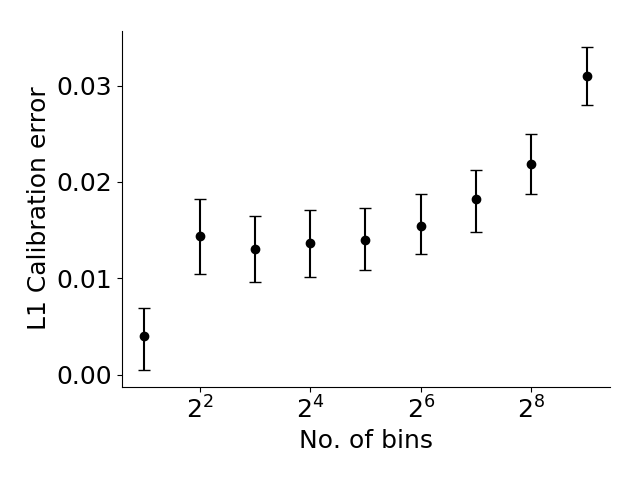
\includegraphics[width=\textwidth]{l1_lower_bound_imagenet_plot}
         \caption{ImageNet, $\ell_1\mbox{-CE}$}
         \label{fig:imagenet_lower_bound_l1}
     \end{subfigure}
     \hfill
     \begin{subfigure}[b]{0.45\textwidth}
         \centering
         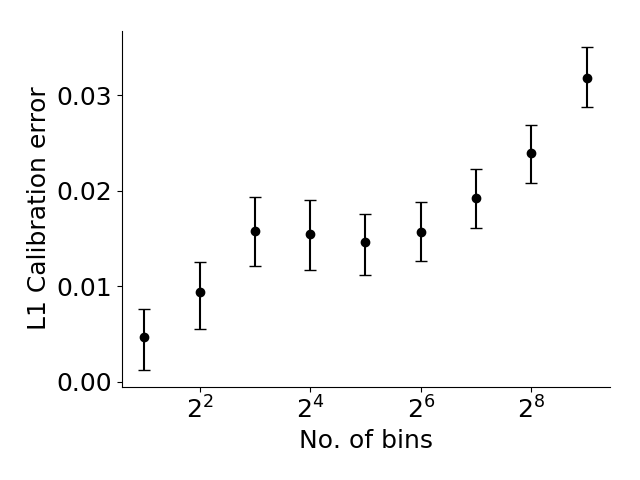
\includegraphics[width=\textwidth]{l1_lower_bound_imagenet_plot_prob_bin}
         \caption{ImageNet, $\ell_1\mbox{-CE}$, equal-probability binning}
         \label{fig:imagenet_lower_bound_l1_prob}
     \end{subfigure}
        \caption{
        Binned $\ell_1$ calibration errors of a recalibrated VGG-net model on ImageNet with $90\%$ confidence intervals. The binned calibration error increases as we increase the number of bins. This suggests that binning cannot be reliably used to measure the $\ell_1\mbox{-CE}$.
        }
        \label{fig:lower_bounds_l1_imagenet}
\end{figure}

We repeated both of these experiments on CIFAR-10 as well, and plot the results in Figure~\ref{fig:lower_bounds_l1_cifar}. Here the results are inconclusive because the error bars are large. This is because the CIFAR-10 dataset is smaller than ImageNet, and the accuracy of the CIFAR-10 model is 93.1\%, so the calibration error that we are trying to measure is much smaller.

\begin{figure}
     \centering
     \begin{subfigure}[b]{0.45\textwidth}
         \centering
         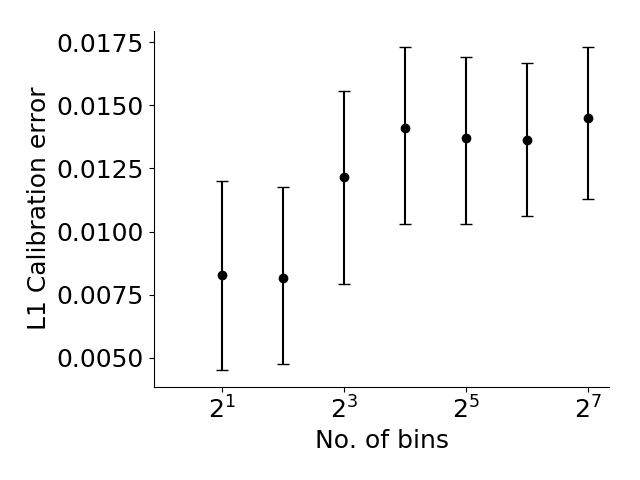
\includegraphics[width=\textwidth]{l1_lower_bound_cifar_plot}
         \caption{CIFAR-10, $\ell_1\mbox{-CE}$}
         \label{fig:cifar_lower_bound_l1}
     \end{subfigure}
     \hfill
     \begin{subfigure}[b]{0.45\textwidth}
         \centering
         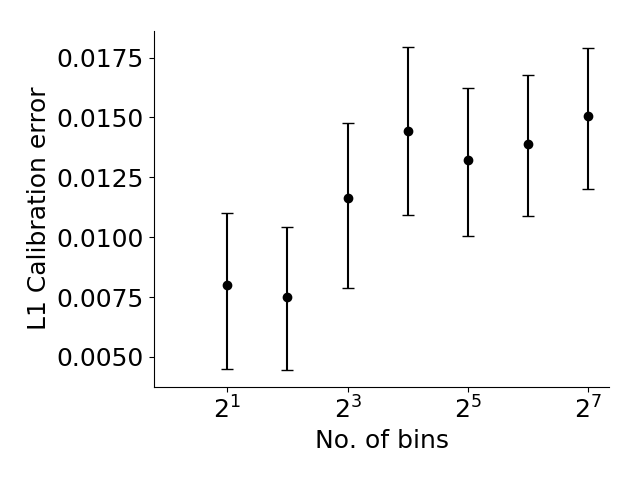
\includegraphics[width=\textwidth]{l1_lower_bound_cifar_plot_prob_bin}
         \caption{CIFAR-10, $\ell_1\mbox{-CE}$, equal-probability binning}
         \label{fig:cifar_lower_bound_l1_prob}
     \end{subfigure}
        \caption{
        Binned $\ell_1$ calibration errors of a recalibrated VGG-net model on CIFAR-10 with $90\%$ confidence intervals. The results are not as conclusive here because the error bars are large, however it seems to suggest that the binned calibration error increases as we increase the number of bins.
        }
        \label{fig:lower_bounds_l1_cifar}
\end{figure}

We provide details on the dataset split for CIFAR-10. For CIFAR-10, we used a VGG16 model and split the test set into 3 sets of size $(1000, 1000, 8000)$, where used the first set of data to recalibrate the model using Platt scaling, the second to select the binning scheme, and the third to measure the binned calibration error. As stated in the main body of the paper, for ImageNet we used a split of $(20000, 5000, 25000)$


\section{Proofs for section~\ref{sec:challenges-measuring}}
\label{sec:appendix-platt-not-calibrated}

% \begin{example}
% For any binning scheme $\mathcal{B}$ and $p \in \mathbb{Z}^+$, there exists a distribution $P$ over $X, Y$ and a function f s.t. $\ell_p\mbox{-CE}(f, B) = 0$ but $\ell_p\mbox{-CE}(f, B) = 0.5$. Note that the $\ell_p\mbox{-CE}$ is always between 0 and 1.
% \end{example}

\continuousNotCalibrated*

\begin{proof}
As stated in the main text, the intuition is that in each interval $I_j$ in $\bins{}$, the model could underestimate the true probability $\expect[Y \mid f(X)]$ half the time, and overestimate the probability half the time. So if we average over the entire bin the model appears to be calibrated, even though it is very uncalibrated. The proof simply formalizes this intuition.

Since $f$ is bijective and continuous we can select data distribution $P$ s.t. $f(X) \sim \mbox{Uniform}[0.5 - \epsilon, 0.5 + \epsilon]$ for any $\epsilon > 0$. To see this, first note that from real analysis since $f : [0, 1] \to [0, 1]$ and $f$ is bijective and continuous, $f^{-1}$ is also bijective and continuous. That is, $f$ is a homeomorphism. Now, consider $I = f^{-1}([0.5 - \epsilon, 0.5 + \epsilon])$. We will choose $P(X)$ s.t. $P(X \not\in I) = 0$ and $P(X \leq f^{-1}(0.5 - \epsilon + t)) = \frac{t}{2\epsilon}$ for $0 \leq t \leq 2 \epsilon$. Since $f$ is increasing and $f^{-1}$ is continuous, this defines a valid probability distribution, and by construction $f(X) \sim \mbox{Uniform}[0.5 - \epsilon, 0.5 + \epsilon]$.

Now, consider each interval $I_j$ in binning scheme $\bins{}$. Let $p_j = \expect[f(X) \mid f(X) \in I_j]$. Since $f(X) \in [0.5 - \epsilon, 0.5 + \epsilon]$, $p_j \in [0.5 - \epsilon, 0.5 + \epsilon]$ as well. We will choose $P(Y)$ so that $Y$ is $1$ whenever $f(X)$ lands in the first $p_j$ fraction of interval $I_j$, and $0$ whenever $f(X)$ lands in the latter $1 - p_j$ fraction of $I_j$. Then $\expect[Y \mid f(X) \in I_j] = p_j$, so the binned calibration error is 0. But notice that for all $s \in [0.5 - \epsilon, 0.5 + \epsilon]$:
\[ \lvert \expect[Y \mid f(X) = s] - s \rvert \geq 0.5 - \epsilon \]
That is, at every point the model is actually very miscalibrated because $\expect[Y \mid f(X) = s]$ is either $0$ or $1$ while $s \in [0.5 - \epsilon, 0.5 + \epsilon]$. By taking $\epsilon$ very small, we then get that $\lpce(p) \geq 0.5 - \epsilon'$ for any $\epsilon' > 0$, which completes the proof.
\end{proof}


\binningLowerBound*

\begin{proof}
It suffices to prove the claim for the $\ell_p^p$ error:
\[ (\ell_p\mbox{-CE}(f, \bins{}))^p \leq (\ell_p\mbox{-CE}(f, \bins{}'))^p \leq (\ell_p\mbox{-CE}(f))^p \]
This is because if $p > 0$ then $a \leq b \Leftrightarrow a^p \leq b^p$.

For $p \geq 1$, let $l(a, b) = (|a - b|)^p$.
We note that $l$ is convex in both arguments.
The proof is now a simple result of Jensen's inequality and convexity of $l$.

We begin with the first inequality. Suppose that $\mathcal{B}$ is given by intervals $I_1, ..., I_m$. Let $Z = f(X)$. Note that $Z$ is a random variable.

% We begin with the first inequality.
% Let $Z = f(X)$, and let $J'$ be the bin in $\bins{}'$ $Z$ lands in, that is $Z \in I_{J'}'$.
% Note that $Z$ and $J'$ are random variables.
% The definition of $(\ell_p\mbox{-CE}(f, \bins{}))^p$ is:
% \[ (\ell_p\mbox{-CE}(f, \bins{}))^p = \sum_{j=1}^m P(Z \in I_j) \; l \Big( \mathbb{E}[Z | Z \in I_{J}], \mathbb{E}[Y | Z \in I_{J}] \big] \Big) \]
% Since $\bins{}'$ is finer than $\bins{}$, for every $j$ there exists some $S_j$ s.t. $I_j = \bigcup_{s \in S_j} I_s'$. Also, note that the intervals in a binning scheme are all disjoint. Therefore, we can use the law of total expectation to write $(\ell_p\mbox{-CE}(f, \bins{}))^p$ as:
% \[ (\ell_p\mbox{-CE}(f, \bins{}))^p = \sum_{j=1}^m P(Z \in I_j) \; l \Big( \mathbb{E}_{J' | Z \in I_j} \big[ \mathbb{E}[Z | Z \in I_{J'}'] \big], \mathbb{E}_{J' | Z \in I_j} \big[ \mathbb{E}[Y | Z \in I_{J'}'] \big] \Big) \]
% Where all we did was to expand the inner most expectations.
% Next, the definition of $(\ell_p\mbox{-CE}(f, \bins{}'))^p$ is:
% \[ (\ell_p\mbox{-CE}(f, \bins{}))^p = \sum_{j=1}^n P(Z \in I_j') \; l \Big( \mathbb{E}[Z | Z \in I_{J}'], \mathbb{E}[Y | Z \in I_{J}'] \big] \Big) \]
% By using the law of total expectation, we can write $(\ell_p\mbox{-CE}(f, \bins{}'))^p$ as:
% \[ (\ell_p\mbox{-CE}(f, \bins{}))^p = \sum_{j=1}^m P(Z \in I_j) \; \mathbb{E}_{J' | Z \in I_j} \Big[ l\Big( \mathbb{E}[Z | Z \in I_{J'}'], \mathbb{E}[Y | Z \in I_{J'}'] \Big) \Big] \]


Fix bin $I_j \in \bins{}$.
Since $\bins{}'$ is finer than $\bins{}$, there exists some $S_j$ s.t. $I_j = \bigcup_{s \in S_j} I_s'$.

Define the following notation to simplify the proof.
\[ p_s = P(Z \in I_s' | Z \in I_j) \]
\[ f_s = \mathbb{E}[Z | Z \in I_s']\]
\[ y_s = \mathbb{E}[Y | Z \in I_s']\]
Since $I_j = \bigcup_{s \in S_j} I_s'$ and the intervals are disjoint, we have:
\[ \sum_{s \in S_j} p_s = 1 \]
We can write $(\ell_p\mbox{-CE}(f, \bins{}))^p$ and $(\ell_p\mbox{-CE}(f, \bins{}'))^p$ as a weighted sum of the errors in each bin $I_j$.
\[ (\ell_p\mbox{-CE}(f, \bins{}))^p = \sum_{j=1}^m P(Z \in I_j) \; l\Big( \big( \sum_{s \in S_j} p_s f_s \big), \big( \sum_{s \in S_j} p_s y_s \big) \Big) \]
\[ (\ell_p\mbox{-CE}(f, \bins{}'))^p = \sum_{j=1}^m P(Z \in I_j) \Big( \sum_{s \in S_j} p_s l(f_s, y_s) \Big) \]
Then by Jensen's inequality, from the convexity of $l$,
\[ l\Big( \big( \sum_{s \in S_j} p_s f_s \big), \big( \sum_{s \in S_j} p_s y_s \big) \Big) \leq \sum_{s \in S_j} p_s l(f_s, y_s)  \]
Since this inequality holds for each term in the sum, it holds for the whole sum:
\[ (\ell_p\mbox{-CE}(f, \bins{}))^p \leq (\ell_p\mbox{-CE}(f, \bins{}'))^p \]

The proof of the second inequality, that $(\ell_p\mbox{-CE}(f, \bins{}'))^p \leq (\ell_p\mbox{-CE}(f))^p$, closely parallels the first.

Fix some bin $I_j' \in \bins{}'$. We can write $(\ell_p\mbox{-CE}(f, \bins{}'))^p$ as:
\[ (\ell_p\mbox{-CE}(f, \bins{}'))^p = \sum_{j=1}^n P(Z \in I_j') \; l\Big( \mathbb{E}[Z | Z \in I_j'], \mathbb{E}[Y | Z \in I_j'] \Big) \]
We can write $(\ell_p\mbox{-CE}(f))^p$ as:
\[ (\ell_p\mbox{-CE}(f))^p = \sum_{j=1}^n P(Z \in I_j) \; \mathbb{E}\Big[ l\big( Z, \mathbb{E}[Y | Z] \big) \; | \; Z \in I_j' \Big] \]
By Jensen's inequality,
\[ l\Big( \mathbb{E}[Z | Z \in I_j'], \mathbb{E}[Y | Z \in I_j'] \Big) \leq \mathbb{E}\Big[ l\big( Z, \mathbb{E}[Y | Z] \big) \; | \; Z \in I_j' \Big] \]
Since this inequality holds for each term in the sum, it holds for the whole sum:
\[ (\ell_p\mbox{-CE}(f, \bins{}'))^p \leq (\ell_p\mbox{-CE}(f))^p \]
\end{proof}


\newpage
\section{Proofs for section~\ref{sec:calibrating_models}}
\label{sec:calibrating_models_appendix}

\newcommand{\G}[0]{\ensuremath{\mathcal{G}}}

Our analysis of the sample complexity of \ourcal{} requires some assumptions on the function family $\G{}$:

\begin{enumerate}
\item (Finite parameters). Let $\G{} = \{ g_{\theta} : \mathcal{Z} \to [0, 1] \; | \; \theta \in A \}$ where $A \subseteq \mathbb{R}^{d}$ and $A$ is open.
\item (Injective). For all $g_{\theta} \in \G{}$ we assume $g_{\theta}$ is injective.
\item (Consistency) Intuitively, consistency means that given infinite data, the estimated parameters should converge to the unique optimal parameters in $A$.
More formally, suppose $\theta^* = \argmin_{\theta \in A} \mse(g_{\theta})$.
Then the parameters $\hat{\theta}_n$ estimated by minimizing the empirical MSE with $n$ samples in step 1 of the algorithm, converges in distribution to $\theta^*$, that is, $\hat{\theta}_n \to_D \theta^*$ as $n \to \infty$. Note that consistency inherently assumes identifiability, that there is a unique minimizer $\theta^*$ in the open set $A$.
\item (Regularity). We assume that regularity conditions in Theorem 5.23 of~\cite{vaart98asymptotic} hold, which require the loss to be twice differentiable with symmetric, non-singular Hessian, and that $g_{\theta}(x)$ is Lipschitz in $\theta$ for all $x$. We will also require the second derivative to be continuous.
\end{enumerate}

We assume that $\G{}$ satisfies these assumptions in the rest of this section. Note that aside from injectivity, the remaining conditions are only required for the (fairly standard) analysis of step 1 of the algorithm, which says that a parametric scaling method with a small number of parameters will quickly converge to its optimal error.

% We first need to introduce the Bayes optimal recalibrator $\omega^*$, which we compare all other recalibrators to. $\omega^* \circ f$ has calibration error $0$, and also has the minimum mean-squared error among all recalibrators.

% \begin{definition}
% $\omega^* : \mathcal{Z} \to [0, 1]$ is given by $\omega^*(x) = \expect[Y | Z = z]$.
% \end{definition}

\subsection{Calibration bound (Proof of Theorem~\ref{thm:final-calib})}

The goal is to prove the following theorem from Section~\ref{sec:calibrating_models}, which we restate:

\begin{finalCalib}
\finalCalibText{}
\end{finalCalib}


We will analyze each step of our algorithm and then combine the pieces to get Theorem~\ref{thm:final-calib}.
As we mention in the main text, step 3 is the main step, so Lemma~\ref{thm:empirical-binning} is one of the core parts of our proof.
Step 2 is where we construct a binning scheme so that each bin has an equal number of points---we show that this property holds approximately in the population (Lemma~\ref{lem:well-balanced}).
This is important as well, particularly to ensure we can estimate the calibration error.
Step 1 is basically Platt scaling, and the asymptotic analysis is fairly standard.

\textbf{Step 3}: Our proofs will require showing convergence in $\ell_2$ and $\ell_1$ norm in function space, which we define below:

\begin{definition}[Distances between functions]
Given $f, g : \mathcal{Z} \to [0, 1]$, for the $\ell_2$ norm we define $||f - g||_2^2 = \expect[(f(Z) - g(Z))^2]$ and $||f- g||_2 = \sqrt{||f - g||_2^2}$. For the $\ell_1$ norm we define $||f - g||_1 = \expect[\lvert f(Z) - g(Z)\rvert]$
\end{definition}

Recall that we showed that in the limit of infinite data the binned version of $g$, $g_{\bins{}}$, has lower calibration error than $g$ (Proposition~\ref{prop:bin_low_bound}). However our method uses $n$ data points to empirically bin $g$, giving us $\hat{g_{\bins{}}}$. We now show the key lemma that allows us to bound the calibration error and later the mean-squared error. That is, we show that the empirically binned function $\hat{g_{\bins{}}}$ quickly converges to $g_{\bins{}}$ in both $\ell_2$ and $\ell_1$ norms.

\begin{lemma}[Empirical binning]
\label{thm:empirical-binning}
There exist constants $c_B, c_1, c_2$ such that the following is true. Given $g : \mathcal{Z} \to [0, 1]$, binning set $T_3 = \{(z_i, y_i)\}_{i=1}^n$ and a 2-well-balanced binning scheme $\bins{}$ of size $B$. Given $0 < \delta < 0.5$, suppose that $n \geq c_B B\log{\frac{B}{\delta}}$. Then with probability at least $1 - \delta$,  $||\hat{g_{\bins{}}} - g_{\bins{}}||_2 \leq \frac{c_2}{\sqrt{n}}\sqrt{\log{\frac{B}{\delta}}}$ and $||\hat{g_{\bins{}}} - g_{\bins{}}||_1 \leq \frac{c_1}{\sqrt{nB}}\sqrt{\log{\frac{B}{\delta}}}$
\end{lemma}

\begin{proof}
% Note, for the L2 bound we only need 1 side of 2-well-balanced, P(f(X) \in I_j) \geq 1/2B for all j.
% For the L1 bound, if we have only 1 side of 2-well-balanced, but b_j - b_{j-1} are equal for all j, then we get the same bound.
% One question is whether we can relax this theorem, for example if b_j - b_{j-1} are equal for all j. Maybe we don't need well-balancedness in that case.
% We first discuss high level intuition for the proof. Recall that in the naive binning approach, where we bin the label (that is, $Y$) values, the $\ell_2$ calibration error is $O(\sqrt{\frac{B}{n}})$ ignoring $\log$ factors. That is, the number of samples we need for calibration increases linearly with the number of bins. The intuition is that when we have more bins, we have fewer samples per bin. That is, we have $\frac{n}{B}$ samples of $Y$ in each bin, where $Y \in \{0, 1\}$. Then Hoeffding's bound gives us the above result, which is tight up to constants. However, this theorem shows when we bin $f$ instead of $Y$, our rates have much better dependencies on $B$. The high level idea is that for each bin $j$ we are taking the average of values bounded in $I_j = [b_{j-1}, b_j]$. This is a narrower range than in naive binning where we took the average of values in $\{0, 1\}$. Since the values are bounded in a narrower range, the variance is lower. Of course, the variance of any particular bin could be big. For example we could have $I_7 = [0.1, 0.9]$. But the sum of all the bin sizes is 1, so `most' of the bins have a lower variance. We now give the formal proof.

Recall that the intuition is in Figure~\ref{fig:variance_reduced_illustration} of the main text---the $g(z_i)$ values in each bin (gray circles in Figure~\ref{fig:var_red_binning}) are in a narrower range than the $y_i$ values (black crosses in Figure~\ref{fig:hist_binning}) so when we take the average we incur less of an estimation error. Now, there may be a small number of bins where the $g(z_i)$ values are not in a narrow range, but we will use the assumption that $\bins{}$ is 2-well-balanced to show that these effects average out and the overall estimation error is small.

Define $R_j$ to be the set of $g(z_i)$ that fall into the $j$-th bin, given by $R_j = \{g(z_i) \mid g(z_i) \in I_j \wedge (z_i, y_i) \in T_3\}$ (recall that $T_3$ is the data we use in step 3).
Let $p_j$ be the probability of landing in bin $j$, given by $p_j = \prob(g(Z) \in I_j)$.
Since $\bins{}$ is 2-well-balanced, $p_j \geq \frac{1}{2B}$.
Since $n \geq c_B B\log{\frac{B}{\delta}}$, by the multiplicative Chernoff bound, for some large enough $c_B$, with probability at least $1 - \frac{\delta}{2}$, $|R_j| \geq \frac{p_j}{2}$.

Consider each bin $j$. Let $\mu_j$ be the expected output of $g$ in bin $j$, given by $\mu_j = \expect[g(Z) \; | \; g(Z) \in I_j]$. $\mu(R_j)$, the mean of the values in $R_j$, is the empirical average of $|R_j|$ such values, each bounded between $b_{j-1}$ and $b_j$ where $I_j = [b_{j-1}, b_j]$. So $\hat{\mu}(R_j)$ is sub-Gaussian with parameter:

\[ \sigma^2 = \frac{(b_j - b_{j-1})^2}{4|R_j|} \leq \frac{(b_j - b_{j-1})^2}{2p_jn} \]

Then by the sub-Gaussian tail bound, for any $1 \leq j \leq B$, with probability at least $1 - \frac{\delta}{2B}$, we have:
\begin{align} (\mu_j - \hat{\mu}(R_j))^2 \leq \frac{(b_j - b_{j-1})^2}{p_jn} \log{\frac{4B}{\delta}}\label{eqn:1} \end{align}

So by union bound with probability at least $1 - \frac{\delta}{2}$ the above holds for all $1 \leq j \leq B$ simultaneously.

We then bound the $\ell_2$-error.
\begin{align*}
||\hat{g_{\mathcal{B}}} - g_{\mathcal{B}}||_2 &= \sqrt{\sum_{j =1}^B p_j (\mu_j - \hat{\mu}(R_j))^2} \\
&\leq \sqrt{\sum_{j =1}^B p_j \frac{(b_j - b_{j-1})^2}{p_jn} \log{\frac{4B}{\delta}}} \tag{by equation~\eqref{eqn:1}}\\
&= \sqrt{\frac{1}{n} \log{\frac{4B}{\delta}} \sum_{j =1}^B (b_j - b_{j-1})^2 } \\
&\leq \sqrt{\frac{1}{n} \log{\frac{4B}{\delta}} \sum_{j =1}^B (b_j - b_{j-1}) } \tag{because $0\le b_j - b_{j-1}\le 1$}\\
&\leq \sqrt{\frac{1}{n} \log{\frac{4B}{\delta}} } \\
&\leq c_2 \frac{1}{\sqrt{n}} \sqrt{\log{\frac{B}{\delta}}}
\end{align*}

Similarly, we can also bound the $\ell_1$-error. Here we also use the fact that $p_j \leq \frac{2}{B}$ since $\bins{}$ is 2-well-balanced.
\begin{align*}
||\hat{g_{\mathcal{B}}} - g_{\mathcal{B}}||_1 &= \sum_{j =1}^B p_j |\mu_j - \hat{\mu}(R_j)| \\
&\leq \sum_{j =1}^B p_j \sqrt{\frac{(b_j - b_{j-1})^2}{p_jn} \log{\frac{4B}{\delta}}} \\
&=\sum_{j =1}^B \sqrt{\frac{p_j(b_j - b_{j-1})^2}{n} \log{\frac{4B}{\delta}}} \\
&\leq \sum_{j =1}^B \sqrt{\frac{2(b_j - b_{j-1})^2}{Bn} \log{\frac{4B}{\delta}}} \\
&\leq \sqrt{\frac{2}{Bn} \log{\frac{4B}{\delta}}} \sum_{j =1}^B (b_j - b_{j-1}) \\
&\leq c_1 \frac{1}{\sqrt{Bn}} \sqrt{\log{\frac{B}{\delta}}}
\end{align*}
By union bound, these hold with probability at least $1 - \delta$, which completes the proof.
\end{proof}

\textbf{Step 2}: Recall that we chose our bins so that each bin had an equal proportion of points in the recalibration set. In our proofs we required that this property (approximately) holds in the population as well. The following lemma shows this.

\begin{wellBalanced}
\wellBalancedText{}
\end{wellBalanced}

\begin{proof}
Suppose we are given a bin construction set of size $n$, $T_n = \{(z_1, y_1), \dots, (z_n, y_n)\}$.
% We want to show that if an interval $I_j$ contains $\frac{n}{B}$ points $g(z_i)$ then $\frac{1}{2B} \leq \prob(g(Z) \in I_j) \leq \frac{2}{B}$.
For any interval $I$, let $\hat{P}(I)$ be the empirical estimate of $P(I) = \prob(g(Z) \in I)$ given by:
\[ \hat{P}(I) = \frac{|\{(z_i, y_i) \in T_n \mid g(z_i) \in I\}|}{n} \]

We constructed the bins so that each interval $I_j$ contains $\frac{n}{B}$ points, or in other words, $\hat{P}(I_j) = \frac{1}{B}$. We want to show that $\frac{1}{2B} \leq \prob(g(Z) \in I_j) \leq \frac{2}{B}$. Since the intervals are chosen from data, we want a uniform concentration result that holds for all such intervals $I_j$.

We will use a discretization argument. The idea is that we will cover $[0, 1]$ with $10B$ disjoint small intervals such that for each of these intervals $I_j'$, $P(g(Z) \in I_j') = \frac{1}{10B}$. We will then use Bernstein and union bound to get that with probability at least $1 - \delta$, for all $I_j'$, $|P(I_j') - \hat{P_j}(I_j')| \leq \frac{1}{100B}$ . Given an arbitrary interval $I$, we can write it as an approximate union of these small intervals, which will allow us to concentrate $|P(I) - \hat{P}(I)|$.

\textbf{Concentrating the small intervals:} Fix some interval $I_j'$. Let $w_i = \mathbb{I}(g(z_i) \in I_j')$ for $i = 1,\dots,n$. Then $w_i \sim \mbox{Bernoulli}(\frac{1}{10B})$. $\hat{P}(I_j')$ is simply the empirical average of $n$ such values and as such with probability at least $1 - \frac{\delta}{10B}$:
\[ |P(I_j') - \hat{P_j}(I_j')| \leq \sqrt{\frac{2}{10Bn} \log{\frac{10B}{\delta}}} + \frac{2}{3n} \log{\frac{10B}{\delta}} \]
If $n = cB \log{\frac{B}{\delta}}$ for a large enough constant $c$, we get:
\[ |P(I_j') - \hat{P_j}(I_j')| \leq \frac{1}{100B} \]
And this was with probability at least $1 - \frac{\delta}{10B}$. So by union bound we get that with probability at least $1 - \delta$ this holds for all $I_j'$.

\textbf{Concentrating arbitrary intervals:} Now consider arbitrary $I \subseteq [0, 1]$. We can approximately write $I$ as a union of the small $I_j'$ intervals. More concretely, we can form a lower bound for $\hat{P}(I)$ by considering all $I_j'$ contained in $I$:
\[ S_L = \{I_j' \mid I_j' \subseteq I \} \]
Similarly we can form an upper bound for $\hat{P}(I)$ by considering all $I_j'$ that have non-empty intersection with $I$:
\[ S_U = \{I_j' \mid I_j' \cap I \neq \emptyset \} \]
We can then show:
\[  \frac{9}{10} P(I) - \frac{1}{5B} \leq \hat{P}(I) \leq \frac{11}{10} P(I) + \frac{1}{5B} \]
Since in our case for all $j$, $\hat{P}(I_j) = \frac{1}{B}$, this gives us:
\[ \frac{1}{2B} \leq P(I_j) \leq \frac{2}{B} \]
\end{proof}

\textbf{Step 1}: Recall that step 1 essentially applies a scaling method---we fit a small number of parameters to the recalibration data.
We show that if $\G{}$ contains $g^* \in \G{}$ with low calibration error, then the empirical risk minimizer $g \in \G{}$ of the mean-squared loss will also quickly converge to low calibration error.
Intuitively, methods like Platt scaling fit a single parameter to the data so standard results in asymptotic statistics tell us they will converge quickly to their optimal error, at least in mean-squared error.
We can combine this with a decomposition of the mean-squared error into calibration and refinement, and the injectivity of $g \in \mathcal{G}$, to show they also converge quickly in calibration error.

\begin{lemma}[Convergence of scaling]
\label{lem:platt_scaling_bound}
Given $\delta$, there exists a constant $c$, such that for all $n$, $\squaredce(g) \leq \min_{g' \in \G{}}\squaredce(g') + \frac{c}{n}$, with probability at least $1 - \delta$.
% independent of $d, L, n$ such that with high probability over the recalibration samples $\squaredce(g) \leq \min_{g' \in \G{}}\squaredce(g') + \frac{cLd \log{R}}{\sqrt{n}}$, where recall that $g \in \G{}$ was selected as the empirical risk minimizer of the mean-squared error loss.
\end{lemma}

\begin{proof}

\textbf{From calibration error to mean-squared error}: We use the classic decomposition of the mean-squared error into calibration error (also known as reliability) and refinement\footnote{Note that the refinement term can be further decomposed into resolution (also known as sharpness) and irreducible uncertainty.}. For any $g \in \G{}$ we have:
\[ \mse(g) = \underbrace{\squaredce(g)}_{\mbox{calibration}} + \underbrace{\expect[(\expect[Y \mid g(Z)] - Y)^2]}_{\mbox{refinement}} \]
Note that the refinement term is constant for all injective $g \in \G{}$, since for injective $g$:
\[ \expect[(\expect[Y \mid g(Z)] - Y)^2] = \expect[(\expect[Y \mid Z] - Y)^2] \]
This means that the difference in calibration error between any $g$ and $g'$ is precisely the difference in the mean-squared error. So it suffices to upper bound the generalization gap $\mse(g) - \mse(g^*)$ for the mean-squared error. Our analysis is fairly standard: we will show asymptotic convergence in the parameter space, and then use a Taylor expansion to show convergence in the MSE loss.

\textbf{Parameter convergence}: Recall that $\hat{\theta}$ denotes the parameters estimated by optimizing the empirical mean-squared error objective on $n$ samples in step 1 of our algorithm, and $\theta^*$ denotes the optimal parameters that minimize the mean-squared error objective on the population. From Theorem 5.23 of~\cite{vaart98asymptotic}, on the asymptotic parameter convergence of M-estimators, we have as $n \to \infty$:
\[ \sqrt{n}(\hat{\theta} - \theta^*) \to_D N(0, \Sigma) \]
Then for each $1 \leq i \leq d$, we have:
\[ \sqrt{n}(\hat{\theta}_i - \theta^*_i) \to_D N(0, \sigma_i^2) \]
We will show that there exists $c_i$ such that for each $i$ and for all $n$, with probability at least $1 - \frac{\delta}{d}$:
\[ \lvert \hat{\theta}_i - \theta^*_i \rvert \leq \frac{c_i}{n} \]
To see this, we begin with the definition of convergence in distribution, which says that the CDFs converge pointwise at every point where the CDF is continuous, which for a Gaussian is every point. That is, letting $z_i$ be a sample from $N(0, \sigma_i^2)$, we have for all $c$:
\[ \lim_{n \to \infty} \prob( \sqrt{n}(\hat{\theta}_i - \theta^*_i) \geq c) = \prob(z_i \geq c) \]
By considering the CDF at each point and its negative, we can show the same result for the absolute value:
\[ \lim_{n \to \infty} \prob( \sqrt{n} \lvert \hat{\theta}_i - \theta^*_i \rvert \geq c) = \prob(\lvert z_i \rvert \geq c) \]
The tails of a normal distribution are bounded, so we can choose $c_i'$ such that:
\[ \prob(\lvert z_i \rvert \geq c_i') \leq \frac{\delta}{2d} \]
By definition of limit, this means that we can choose $N_i$ such that for all $n \geq N_i$, we have:
\[ \prob( \sqrt{n} \lvert \hat{\theta}_i - \theta^*_i \rvert \geq c_i') \leq \frac{\delta}{d} \]
In other words, for all $n \geq N_i$, with probability at least $1 - \frac{\delta}{d}$:
\[ \lvert \hat{\theta}_i - \theta^*_i \rvert \leq \frac{c_i'}{\sqrt{n}} \]
Since this only does not hold for finitely many values $1, \cdots, N_i - 1$, we can `absorb' these cases into the constant. That is, for each $n \in \{1, \cdots, N_i - 1 \}$, there exists $r_n$ such that if we use $n$ samples, then except with probability $\frac{\delta}{d}$, $\lvert \hat{\theta}_i - \theta^*_i \rvert \leq r_n$. So then we can choose $c_i$ such that for all $n$:
\[ \lvert \hat{\theta}_i - \theta^*_i \rvert \leq \frac{c_i' + \max_{1 \leq m < N_i}{r_m \sqrt{m}}}{\sqrt{n}} \leq \frac{c_i}{\sqrt{n}} \]
We apply union bound over the indices $i$, and can then bound the $\ell_2$-norm of the difference between the estimated and optimal parameters, so that we can choose $k$ such that for all $n$, with probability at least $1 - \delta$:
\[ ||\hat{\theta} - \theta^*||_2^2 \leq \frac{k}{n} \]

\textbf{Loss convergence}: We denote the loss by $L$, defined as:
\[ L(\theta) = \mse(g_{\theta}) = \expect[ (Y - g_{\theta}(X))^2 ] \]
We approximate the loss $L$ by the first few terms of its Taylor expansion, which we denote by $\widetilde{L}$:
\[ \widetilde{L}(\theta) = L(\theta^*) + \nabla L(\theta^*)^T (\hat{\theta} - \theta^*) + (\hat{\theta} - \theta^*)^T \nabla^2 L(\theta^*) (\hat{\theta} - \theta^*) \]
We assumed that $L$ was twice differentiable with continuous second derivative, and that $\theta^*$ minimized the loss in an open set, so $\nabla L(\theta^*) = 0$, and we also have (see e.g. Theorem 3.3.18 in~\cite{hubbard1998vector}):
\[ \lim_{||\hat{\theta} - \theta^*||_2 \to 0} \frac{L(\hat{\theta}) - \widetilde{L}(\hat{\theta})}{||\hat{\theta} - \theta^*||_2^2} = 0 \]
By the definition of a limit if we fix $\epsilon > 0$, there exists $R > 0$ such that if $||\hat{\theta} - \theta^*||_2 \leq R$ then $L(\hat{\theta}) - \widetilde{L}(\hat{\theta}) \leq \epsilon ||\hat{\theta} - \theta^*||_2^2$. For some large enough $N_0$, if $n \geq N_0$, then with probability at least $1 - \delta$, $||\hat{\theta} - \theta^*||_2 \leq R$. As before, since this only does not hold for finitely many $N$, we can fold these cases into the constant so that there exists $\epsilon'$ such that for all $n$, $L(\hat{\theta}) - \widetilde{L}(\hat{\theta}) \leq \epsilon' ||\hat{\theta} - \theta^*||_2^2$ with probability at least $1 - \delta$. Plugging in $\widetilde{L}(\hat{\theta})$, we have:
\[ L(\hat{\theta}) - L(\theta^*) \leq (\hat{\theta} - \theta^*)^T \nabla^2 L(\theta^*) (\hat{\theta} - \theta^*) + \epsilon' ||\hat{\theta} - \theta^*||_2^2 \]
We can bound this by the operator norm of the Hessian, and then use the parameter convergence result:
\[ L(\hat{\theta}) - L(\theta^*) \leq (|| \nabla^2 L(\theta^*) ||_{op} + \epsilon') ||\hat{\theta} - \theta^*||_2^2 \leq \frac{c}{n} \]
which holds with probability at least $1 - \delta$, as desired.

% From a standard $\epsilon$-cover in the parameter space, or PAC-Bayes argument, we can get a high probability generalization bound on the mean-squared error:
% \[ \mse(g) \leq \mse(g^*) + \frac{cLd \log{R}}{\sqrt{n}} \]
% This gives us the desired result.
\end{proof}

Finally, we have the tools to prove the main theorem:

\begin{proof}[Proof of Theorem~\ref{thm:final-calib}]
The proof pieces together Lemmas~\ref{lem:platt_scaling_bound},~\ref{thm:empirical-binning},~\ref{lem:well-balanced} and Proposition~\ref{prop:bin_low_bound}.

For any fixed $c_1 > 0$, there exists $c_1'$ such that if $n \geq c_1'\big(\frac{1}{\epsilon^2}\big)$, from Lemma~\ref{lem:platt_scaling_bound}, step 1 of our algorithm gives us $g$ with $\squaredce(g) \leq \min_{g' \in \G{}}\squaredce(g') + c_1 \epsilon^2$, with probability at least $1 - \frac{\delta}{3}$.

Next, for universal constant $c_2$, if $n \geq c_2(B \log{\frac{B}{\delta}})$, from Lemma~\ref{lem:well-balanced}, step 2 chooses a 2-well-balanced binning scheme $\bins{}$ with probability at least $1 - \frac{\delta}{3}$.

From Proposition~\ref{prop:bin_low_bound}, $\squaredce(g_{\bins{}}) \leq \squaredce(g) \leq \min_{g' \in \G{}}\squaredce(g') + c_1 \epsilon^2$. Then from Lemma~\ref{thm:empirical-binning}, for any $c_3 > 0$, there exists $c_3'$ such that if $n \geq c_3'\big(\frac{1}{\epsilon^2} \log{\frac{B}{\delta}}\big)$, step 3 gives us $\hat{g_{\bins{}}}$ with $||\hat{g_{\bins{}}} - g_{\bins{}}||_2 \leq c_3 \epsilon$ with probability at least $1 - \frac{\delta}{3}$. We want to say that since $\hat{g_{\bins{}}}$ is close to $g_{\bins{}}$ and $g_{\bins{}}$ has low calibration error, this must mean that $\hat{g_{\bins{}}}$ has low calibration error.

To do this we represent the $\ell_2$ calibration error of any $g$ as the distance between $g$ and a perfectly recalibrated version of $g$. That is, we define the perfectly recalibrated version of $g$ as:
\[ \omega(g)(z) = \expect[ Y \mid g(Z) = z ] \]
Then for any $g$, we can write $\ltwoce(g) = ||g - \omega(g)||_2$. By triangle inequality on the $\ell_2$ norm on functions, we have:
\[ ||\hat{g_{\bins{}}} - \omega(g_{\bins{}})||_2 \leq ||\hat{g_{\bins{}}} - g_{\bins{}}||_2 + ||g_{\bins{}} - \omega(g_{\bins{}})||_2 \leq c_3 \epsilon + \sqrt{\min_{g' \in \G{}}\squaredce(g') + c_1 \epsilon^2} \]

Now the LHS is not quite the $\ell_2$ calibration error of $\hat{g_{\bins{}}}$, which is $||\hat{g_{\bins{}}} - \omega(\hat{g_{\bins{}}})||_2$~\footnote{This is a very technical point, so at a first pass the reader may skip the following discussion.}.
However, since $g$ is injective, $g_{\bins{}}$ takes on a different value for each interval $I_j \in \bins{}$.
If $\hat{g_{\bins{}}}$ also takes on a different value for each interval $I_j \in \bins{}$, then we can see that $\omega(g_{\bins{}}) = \omega(\hat{g_{\bins{}}})$.
If not, $\omega(\hat{g_{\bins{}}})$ can only merge some of the intervals of $\omega(g_{\bins{}})$, and by Jensen's we can show:
\[ ||\hat{g_{\bins{}}} - \omega(\hat{g_{\bins{}}})||_2 \leq ||\hat{g_{\bins{}}} - \omega(g_{\bins{}})||_2 \leq c_3 \epsilon + \sqrt{\min_{g' \in \G{}}\squaredce(g') + c_1 \epsilon^2} \]
An alternative way to see this is to add infinitesimal noise to $\hat{g_{\bins{}}}$ for each interval $I_j$, in which case we get $\omega(g_{\bins{}}) = \omega(\hat{g_{\bins{}}})$.
Finally we convert back from the $\ltwoce$ to $\squaredce$:
\[ \squaredce(\hat{g_{\bins{}}}) = ||\hat{g_{\bins{}}} - \omega(\hat{g_{\bins{}}})||_2^2 \leq \min_{g' \in \G{}}\squaredce(g') + (c_3^2 + c_1) \epsilon^2 + 2\sqrt{(c_3^2 \epsilon^2) \big(\min_{g' \in \G{}}\squaredce(g') + c_1 \epsilon^2\big)} \]
By the AM-GM inequality, we have:
\[ 2\sqrt{(c_3^2 \epsilon^2) \big(\min_{g' \in \G{}}\squaredce(g') + c_1 \epsilon^2\big)} \leq (c_3^2 + c_1) \epsilon^2 + \min_{g' \in \G{}}\squaredce(g') \]
Combining these, we get:
\[ \squaredce(\hat{g_{\bins{}}}) \leq 2 \min_{g' \in \G{}}\squaredce(g') + 2(c_3^2 + c_1) \epsilon^2 \]
By e.g. choosing $c_1 = 0.1$ and $c_3 = 0.1$, we have $2(c_3^2 + c_1) \leq 1$, which gives us the desired result. By union bound over each step, we have this with probability at least $1 - \delta$.


% From proposition Y, $\twoce(g_{\bins{}}) \leq \ltwoce(g)$
\end{proof}

\subsection{Bounding the mean-squared error}

We also show that if we use lots of bins, discretization has little impact on model quality as measured by the mean-squared error.
Note that recalibration itself typically \emph{reduces/improves} the mean-squared error.
However, in our method after fitting a recalibration function like Platt scaling does, we discretize the function outputs.
This reduces the calibration error and allows us to measure the calibration error, but it does increase the mean-squared error by a small amount.
Here we upper bound the increase in mean-squared error.
In other words, our method allows for the calibration error of the final model to be measured, and has little impact on the mean-squared error.

\begin{restatable}[MSE Bound]{proposition}{mseFiniteBinning}
\label{prop:mse-finite-binning}
If $\mathcal{B}$ is a 2-well-balanced binning scheme of size $B$ and $B = \widetilde{\Omega}(n)$, where $\widetilde{\Omega}$ hides $\log$ factors, then $\mse(\hat{g}_{\mathcal{B}}) \leq \mse(g) + O(\frac{1}{B})$.
\end{restatable}

To show this we begin with a lemma showing that if $f$ and $g$ are close in $\ell_1$ norm, then their mean-squared errors are close:

\begin{lemma}
\label{lem:mse-l1}
For $f, g : \mathcal{Z} \to [0, 1]$, $\mse(f) \leq \mse(g) + 2||f - g||_1$.
\end{lemma}

\begin{proof}
\begin{align*}
\expect[(f(Z) - Y)^2 - (g(Z) - Y)^2] &= \expect[(f(Z) - g(Z))(f(Z) + g(Z) - 2Y)] \\
&\leq \expect[|f(Z) - g(Z)||f(Z) + g(Z) - 2Y|] \\
&\leq \expect[2|f(Z) - g(Z)|] \\
& =2||f-g||_1
\end{align*}
Where the third line followed because $-2 \leq f(Z) + g(Z) - 2Y \leq 2$.
\end{proof}

Next, we show that in the limit of infinite data, if we bin with a well-balanced binning scheme then the MSE cannot increase by much.

\begin{lemma}
\label{thm:bin-sharpness}
Let $\mathcal{B}$ be an $\alpha$-well-balanced binning scheme of size $B$. Then $\mse(g_{\mathcal{B}}) \leq \mse(g) + \frac{2\alpha}{B}$.
\end{lemma}

\begin{proof}
We bound $||g_{\mathcal{B}} - g||_1$ and then use Lemma~\ref{lem:mse-l1}. We use the law of total expectation, conditioning on $\beta(g(Z))$, the bin that $g(Z)$ falls into.
\begin{align*}
||g_{\mathcal{B}} - g||_1 &= \mathbb{E}[|g_{\mathcal{B}}(Z) - g(Z)|] \\
&\leq \mathop{\mathbb{E}}_{\beta(g(Z))} \Big[ \mathop{\mathbb{E}}_{Z | \beta(g(Z))} [ |g_{\mathcal{B}}(Z) - g(Z)| ]\Big]\\
&\leq \mathop{\mathbb{E}}_{\beta(g(Z))} \Big[ b_{\beta(g(Z))} - b_{\beta(g(Z))-1}\Big]
\end{align*}
We now use the fact that $\mathcal{B}$ is $\alpha$-well-balanced.
\begin{align*}
\mathop{\mathbb{E}}_{\beta(g(Z))} \Big[ (b_{\beta(g(Z))} - b_{\beta(g(Z))-1})\Big] &= \sum_{i=1}^B \prob\big(g(Z) \in [b_{\beta(g(Z))-1}, b_{\beta(g(Z))}]\big) (b_{\beta(g(Z))} - b_{\beta(g(Z))-1}) \\
&\leq \sum_{i=1}^B \frac{\alpha}{B} (b_{\beta(g(Z))} - b_{\beta(g(Z))-1}) \\
&\leq \frac{\alpha}{B}
\end{align*}
Finally, from Lemma~\ref{lem:mse-l1}, we get that $\mse(g_{\mathcal{B}}) \leq \mse(g) + \frac{2\alpha}{B}$.
\end{proof}

The above lemma bounds the increase in MSE due to binning in the infinite sample case -- next we deal with the finite sample case and prove proposition~\ref{prop:mse-finite-binning}:

\begin{proof}[Proof of Proposition~\ref{prop:mse-finite-binning}:]
Ignoring all $\log$ factors, from Theorem~\ref{thm:empirical-binning} if $n = \widetilde{\Omega}(B)$, we have $||\hat{g}_{\mathcal{B}} - g_{\mathcal{B}}||_1 = O(\frac{1}{\sqrt{nB}})$. Then from  Lemma~\ref{lem:mse-l1}, $\mse(\hat{g}_{\mathcal{B}}) \leq \mse(g_{\mathcal{B}}) + O(\frac{1}{\sqrt{Bn}}) \leq \mse(g_{\mathcal{B}}) + O(\frac{1}{B})$. From Theorem~\ref{thm:bin-sharpness}, since $\mathcal{B}$ is 2-well-balanced, we have  $\mse(g_{\mathcal{B}}) \leq \mse(g) + O(\frac{1}{B})$. This gives us $\mse(\hat{g}_{\mathcal{B}}) \leq \mse(g) + O(\frac{1}{B})$.
\end{proof}

\subsection{Alternative binning schemes}
\label{sec:alt_binning_schemes}

We note that there are alternative binning schemes in the literature.
For example, the $B$ bins can be chosen as $I_1 = [0, \frac{1}{B}], I_2 = (\frac{1}{B}, \frac{2}{B}], \dots, I_B = (\frac{B-1}{B}, 1]$.
The main problem with this binning scheme is that we may not be able to measure the calibration error efficiently, which is critical.
However, if we choose the bins like this, and are lucky that the binning scheme happens to be 2-well-balanced, we can improve the bounds on the MSE that we proved above.
This motivates alternative hybrid binning schemes, where we try to keep the width of the bins as close to $1/B$ as possible, while ensuring that each bin contains lots of points as well.
We think analyzing what binning schemes lead to the best bounds, and seeing if this can improve the calibration method, is a good direction for future research.



\newpage
\section{Details and ablations for section~\ref{sec:calibrating_models}}
\label{sec:calibrating_models_appendix_experiments}

We begin by giving more experimental details. Note that the code is available in the supplementary folder for completeness.

We detail our experimental protocol for CIFAR-10 first. The CIFAR-10 validation set has 10,000 data points. We sampled, with replacement, a recalibration set of 1,000 points. In our theoretical approach and analysis, we split up these sets into multiple parts. For example, we used the first part for training a function, second part for bin construction, third part for binning. In practice, using the same set for all three steps worked out better, for both histogram binning and our variance-reduced binning approach. We believe that there may be theoretical justification for merging these sets, although we leave that for future work. For the marginal calibration experiment we ran either the variance-reduced calibrator (we fit a sigmoid in the function fitting step) or histogram binning. We calibrated each of the $K$ classes seprately as described in Section~\ref{sec:formulation}, and measured the marginal calibration error on the entire set of 10K points. We repeated this entire procedure 100 times, and computed mean and 90\% confidence intervals.

\begin{figure}
  \centering
  \centering
  	 \begin{subfigure}[b]{0.48\textwidth}
         \centering
         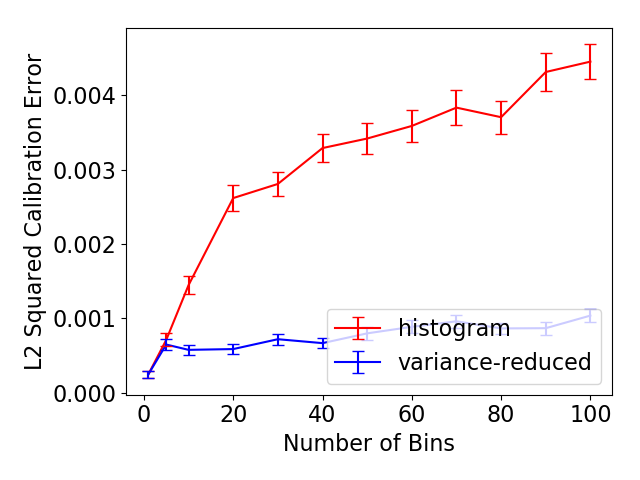
\includegraphics[width=\textwidth]{top_ces_imagenet.png}
         \caption{Effect of number of bins $B$ on top calibration error $\topsquaredce$ on ImageNet.
         }
         \label{fig:imagenet_top_cal_var_red}
     \end{subfigure}
     \hfill
     \begin{subfigure}[b]{0.48\textwidth}
         \centering
         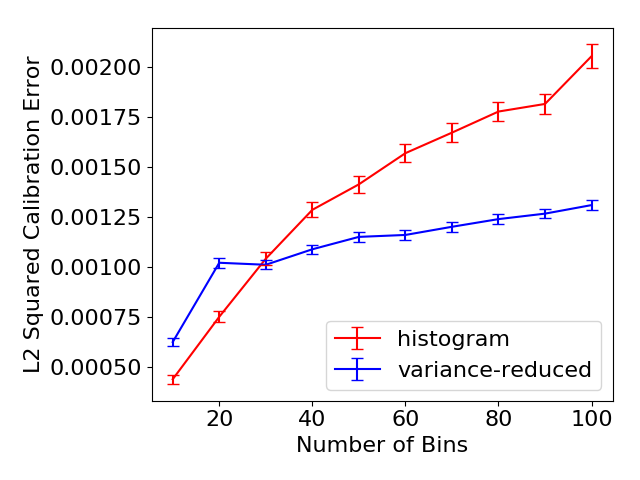
\includegraphics[width=\textwidth]{top_ces_cifar_1000.png}
         \caption{Effect of number of bins $B$ on top calibration error $\topsquaredce$ on CIFAR-10.
         }
         \label{fig:cifar_top_cal_var_red}
     \end{subfigure}
  \caption{
    Recalibrating using 1,000 data points on ImageNet and CIFAR-10, our variance-reduced calibrator typically achieves lower $\ell_2^2$ calibration error than histogram binning, especially when the number of bins $B$ is large. The difference is very significant on ImageNet, where our method does better when $B \geq 10$, and gets a nearly 5 times lower calibration error when $B = 100$. For CIFAR-10 our method does better when $B > 30$, which supports the theory, which predicts that our method does better when $B$ is large. However, when $B$ is small, practitioners should try both histogram binning and the variance-reduced calibrator.
}
  \label{fig:mse_estimators_bins}
\end{figure}

In this experiment, we are checking a very precise hypothesis---assuming that the empirical distribution on the 10,000 validation points is the true data distribution, how do these methods perform? This is similar to the experimental protocol used in e.g.~\cite{brocker2012empirical}.
% This is not the same as an alternative hypothesis---how do these methods perform on the true CIFAR-10 distribution, which we do not have access to.
An alternative experimental protocol would have been to first split the CIFAR-10 data into two sets of size $(1000, 9000)$.
We could have then used the first set to recalibrate the model using either the variance-reduced calibrator or histogram binning, and then used the remaining 9,000 examples to estimate the calibration error on the ground truth distribution, using Bootstrap to compute confidence intervals.
However, when we ran this experiment, we noticed that the results were very sensitive to which set of 1,000 points we used to recalibrate.
Multiple runs of this experiment led to very different results.
The point is that there are two sources of randomness---the randomness in the data the recalibration method operates on, and the randomness in the data used to evaluate and compare the recalibrators.
In our protocol we account for both of these sources of randomness.

We also ran experiments on top-label calibration, for both ImageNet and CIFAR-10. The protocol is exactly as described above, except instead of calibrating each of the $K$ classes, we calibrated the top probability prediction of the model. More concretely, for each input $x_i$, the uncalibrated model outputs a probability $p_i$ corresponding to its top prediction $k_i$, where the true label is $y_i$. We create a new dataset $\{(p_1, \mathbb{I}(k_1 = y_1)), \dots, (p_n, \mathbb{I}(k_n = y_n))\}$ and run our variance-reduced calibration method (fitting a sigmoid in the function fitting step, as in Platt scaling) or histogram binning on this dataset, using $B$ bins. This calibrates the probability corresponding to the top prediction of the model. We evaluate the recalibrated models on the top-label calibration error metric ($\topsquaredce{}$) described in Section~\ref{sec:formulation}. For both CIFAR-10 and ImageNet we sampled, with replacement, a recalibration set of 1,000 points for the recalibration data, and we measured the calibration error on the entire set (10,000 points for CIFAR-10, and 50,000 points for ImageNet) as above. We show $90\%$ confidence intervals for all plots.

Figure~\ref{fig:imagenet_top_cal_var_red} shows that on ImageNet the variance-reduced calibrator gets significantly lower calibration errors than histogram binning when $B \geq 10$, and nearly a 5 times lower calibration error when $B = 100$. Both methods get similar calibration errors when $B = 1$ or $B = 5$. Figure~\ref{fig:cifar_top_cal_var_red} shows that on CIFAR-10 when $B$ is high, the variance-reduced calibrator gets lower calibration errors than histogram binning, but when $B$ is low histogram binning gets lower calibration errors. We believe that the difference might be because the CIFAR-10 model is highly accurate at top-label prediction to begin with, getting an accuracy of over $93\%$, so there is not much scope for re-calibration. In any case, this ablation tells us that practitioners should try multiple methods when recalibrating their models and evaluate their calibration error.


\newpage

\section{Proofs for section~\ref{sec:verifying_calibration}}

\pl{I hope these exist somewhere :-)}

In this section we prove the finite sample bounds for the plugin and canceling estimators. We follow a very similar structure for both the plugin estimator and the canceling estimators.

We first give a proof for the plugin estimator. At a high level, we decompose the plugin estimator into three terms (Lemma~\ref{lem:plugin_decomp}), and then bound each of these terms. Most of these terms simply involve algebraic manipulation and standard concentration results, except Lemma~\ref{lem:p2_bound} which requires some tricky conditioning.

The canceling estimator decomposes into three terms as well, two of these terms are the same as those in the plugin estimator. Bounding the third term (Lemma~\ref{lem:c3_bound}) is the key to the improved sample complexity of the plugin estimator. The canceling estimator is not unbiased. However, with high probability if we condition on the $x_i$s in the evaluation set, each of these error terms is unbiased. We can then use Hoeffding's to concentrate each term near 0. The errors in each bin are then independent which leads to some cancelations of the error terms when we sum them up.

\textbf{We use the following notation simplification} to simplify the theorem statements and proofs:
\[ p_i = P(f(X) = s_i) \]
\[ y_i^* = \mathbb{E}[Y \; | \; f(X) = s_i] \]
\[ e_i = (s_i - y_i^*) \]

Then, if we let ${E^*}^2$ denote the actual $\ell_2^2$ calibration error, we have:
\[ {E^*}^2 = \sum_{i=1}^b p_i e_i^2 \]

% \begin{lemma}
% Suppose $p_i > \piSmallBound{}$ for all $i$. Then except with probability $\delta$ for all $i$ we have:
% \[ |\hat{p_i} - p_i| < \sqrt{\frac{3}{np_i} \log{\frac{2B}{\delta}}} \]
% % For some $k > 1$, suppose $p_i \geq \frac{1}{kb}$ for all $i$. Then if $n \geq 3kb \log{\frac{2b}{\delta}}$, we have $P(\forall i . \; |p_i - \hat{p_i}| \leq c(n) p_i) \geq 1 - \delta$ where
% \end{lemma}

We begin by noting that $\hat{p_i}$ is close to $p_i$ for all $i$. This is a standard application of either Bernstein's inequality or the multiplicative Chernoff bound.

\begin{lemma}
\label{lem:pi_bound}
Suppose $p_i > \piSmallBound{}$ for all $i$. Then we have $c(n) < 0.5$ and except with probability $\delta$ for all $i$ we have:
\[ |\hat{p_i} - p_i| < c(n)p_i = \sqrt{\frac{3}{n \min p_i} \log{\frac{2B}{\delta}}} p_i \]
\end{lemma}

\subsection{Analysis of plugin estimator}

\tm{for appendix, we probably want to maximize clarity. So title could be "Analysis of plugin estimator: proof of Theorem??" }

The following lemma is crucial -- we decompose the plugin estimator into three terms that we can bound separately.

\begin{lemma}[Plugin decomposition]
\label{lem:plugin_decomp}
The plugin estimator satisfies the following decomposition:
\[ \pluginEst{} = \underbrace{\sum_{i=1}^b \hat{p_i}e_i^2}_{(P1)}  - \underbrace{2\sum_{i=1}^b \hat{p_i}e_i(\hat{y_i} - y_i^*)}_{(P2)} + \underbrace{\sum_{i=1}^b \hat{p_i}(\hat{y_i} - y_i^*)^2}_{(P3)} \]
\end{lemma}

\begin{proof}
The proof is by algebra:
\begin{align*}
\pluginEst{} &= \sum_{i=1}^b \hat{p_i}(s_i - \hat{y_i})^2 \\
&= \sum_{i=1}^b \hat{p_i}[e_i - (\hat{y_i} - y_i^*)]^2 \\
&= \underbrace{\sum_{i=1}^b \hat{p_i}e_i^2}_{(P1)}  - \underbrace{2\sum_{i=1}^b \hat{p_i}e_i(\hat{y_i} - y_i^*)}_{(P2)} + \underbrace{\sum_{i=1}^b \hat{p_i}(\hat{y_i} - y_i^*)^2}_{(P3)}
\end{align*}
\end{proof}

We now bound each of these three terms with the following three lemmas. We condition on $|\hat{p_i} - p_i| < c(n)p_i < 0.5p_i$ for all $i$, which holds with high probability from Lemma~\ref{lem:pi_bound}.

\tm{In general, writing proofs is like writing code. lemmas and theorems have type checked inputs and outputs. Inputs are conditiond and definitions, outputs ar conclusions. }
\begin{lemma}[P1]\tm{a better way to write this is probably: Let P1 be defined in equation~\ref{...}}
\label{lem:p1_bound}
Suppose $|\hat{p_i} - p_i| < c(n) p_i$ for all $i$. Then
\[ |(P1) - {E^*}^2| \leq c(n) {E^*}^2 \]
\end{lemma}

\begin{proof}
The proof is by algebra. 
\begin{align*}
|(P1) - {E^*}^2| &= | \sum_{i=1}^b \hat{p_i}e_i^2 - \sum_{i=1}^b p_i e_i^2 | \\
&= | \sum_{i=1}^b (\hat{p_i} - p_i) e_i^2 | \\
&\leq \sum_{i=1}^b |(\hat{p_i} - p_i)| e_i^2 \\
&\leq \sum_{i=1}^b c(n) p_i e_i^2 \\
&\leq c(n) \sum_{i=1}^b p_i e_i^2 \\
&\leq c(n) {E^*}^2
\end{align*}
\end{proof}

\begin{lemma}[P2]\tm{ah maybe I wasn't clear before --- it's not necessary to have this shorthand for all the lemmas and theorems. }
\label{lem:p2_bound}
Suppose $|\hat{p_i} - p_i| < c(n)p_i < 0.5p_i$ for all $i$. Then with probability $\geq 1 - \delta$:
\[ |(P2)| \leq \sqrt{\frac{2(1+c(n)){E^*}^2}{n} \log{\frac{2}{\delta}}} \]
\end{lemma}

\begin{proof}
Recall that we evaluated our estimators on an independent and identically distributed evaluation set $T_n = \{(x_1, y_1), \dots, (x_n, y_n)\}$. Also, note that since $|\hat{p_i} - p_i| < p_i$, $\hat{p_i} > 0$. Let $Z = (f(x_1), \cdots, f(x_n))$ be a random variable. 

$\hat{y_i}$ simply takes the empirical average of the label values, and is therefore an unbiased estimator of $y_i^*$ even if we condition on $Z$:
\[ \expect[\hat{y_i} - y_i^* \mid Z] = 0 \]

Next we look at the distribution of $\hat{y_i} - y_i^* \mid Z$. For all $(x_j, y_j) \in T_n$, $y_j \in \{0, 1\}$. Additionally, $\{y_j \mid (x_j, y_j) \in T_n\} \mid Z$ is also independently (but not identically) distributed. So by Hoeffding's lemma, $\hat{y_i} - y_i^* \mid Z$ is sub-Gaussian with parameter $\frac{1}{4 \hat{p_i} n}$.

Here, we note that $\hat{p_i}$ is a constant given $Z$.
Then, we get that $\hat{p_i}e_i(\hat{y_i} - y_i^*) \mid Z$ has expected value $0$ and is sub-Gaussian with parameter:
\[ \sigma_i^2 = \hat{p_i}^2 e_i^2 \frac{1}{4 \hat{p_i} n} = \frac{\hat{p_i} e_i^2}{4n} \]
This means that the sum, $(P2)$ has expected value $0$ and is sub-Gaussian with  parameter:
\[ \sigma^2 = 2^2 \sum_{i=1}^B \sigma_i^2 = 4 \sum_{i=1}^B \frac{\hat{p_i} e_i^2}{4n} \leq \frac{(1+c(n)){E^*}^2}{n} \]
By applying the sub-Gaussian tail inequality, we get that with probability at least $1-\delta$,
\[ |(P2)| \leq \sqrt{\frac{2(1+c(n)){E^*}^2}{n} \log{\frac{2}{\delta}}} \]
Since this was true for all $Z$, this is true if we marginalize over $Z$ as well, which completes the proof.
\end{proof}

\begin{lemma}[P3]
\label{lem:p3_bound}
Suppose $|\hat{p_i} - p_i| < c(n)p_i < 0.5p_i$ for all $i$. Then with probability $\geq 1 - \delta$:
\[ |(P3)| \leq \frac{B}{2n} \log{\frac{2B}{\delta}} \]
\end{lemma}

\begin{proof}
Fix arbitrary $\hat{p_i}$s satisfying $|\hat{p_i} - p_i| < c(n) p_i < 0.5p_i$. Note that this gives us $\hat{p_i} > 0$.

By Hoeffding's bound, for any fixed $i$, with probability at least $1-\frac{\delta}{b}$:
\[ |\hat{y_i} - y_i^*| \leq \sqrt{\frac{1}{2\hat{p_i}n} \log{\frac{2B}{\delta}}} \]
Applying union bound over $i = 1, \cdots, B$, we get that the above holds \emph{for all $i$} with probability at least $1 - \delta$. Then with probability at least $1 - \delta$, for all $i$:
\[ | \hat{p_i} (\hat{y_i} - y_i^*)^2 | \leq \frac{1}{2n} \log{\frac{2B}{\delta}} \]
Summing over the bins $i = 1, \cdots, B$, we get:
\[ 0 \leq (P3) \leq \frac{B}{2n} \log{\frac{2B}{\delta}}  \]
\end{proof}


Bounding the error of the plugin estimator simply involves combining the bounds for each of the terms, $P1$, $P2$, $P3$.

\pluginBound*

\tm{if you recall a theorem, then need to mark that it's a recall of a previous theorem. e.g., "Restatement of Theorem 5.4"}
\begin{proof}
We have:
\[ |\pluginEst{} - {E^*}^2| \leq |P1 - {E^*}^2| + |P2| + |P3| \]
From Lemma~\ref{lem:pi_bound} we have $|\hat{p_i} - p_i| < c(n)p_i < 0.5p_i$ with probability $\geq 1 - \delta$. Conditioning on this, we combine Lemmas~\ref{lem:p1_bound},~\ref{lem:p2_bound},~\ref{lem:p3_bound} with union bound to get the desired result.
\end{proof}

We then prove the final bound for the plugin estimator.

\finalPlugin*

\begin{proof}
We first provide an intuitive argument, and then a formal proof. When $r = 0.5$, we intuitively want to distinguish between when ${E^*}^2$ is $\epsilon^2$ and $0.5\epsilon^2$. So we want to bound the confidence interval by a constant factor of $\epsilon^2$ in the regime where ${E^*}^2 \approx \epsilon^2$. Substitute ${E^*}^2 = \epsilon^2$ into the bound in Theorem~\ref{thm:plugin-bound}, and write out the condition that $| \pluginEst{} - {E^*}^2 | \leq \frac{\epsilon^2}{4}$. With some simple algebra, we get $n = \Theta(B + \frac{B}{\epsilon})$.

Now we give the formal proof, which formalizes the above intuition. First, we note that if $n \geq 6B \log{\frac{B}{\delta}}$ then $p_i > \piSmallBound{}$ so this satisfies the requirements to apply Theorem~\ref{thm:plugin-bound}.

Let $\omega = \frac{1-r}{2}$. Note that $r + \omega = 1 - \omega$. We split into two cases. In the first case, we will assume that ${E^*}^2 \leq r \epsilon^2$. We will show that with probability at least $1 - \delta$, $\pluginEst{} \leq (1-\omega) \epsilon^2$. In the second case, we will assume that ${E^*}^2 > \epsilon^2$. We will show that with probability at least $1 - \delta$, $\pluginEst{} > (1-\omega) \epsilon^2$. This then gives us an easy way to hypothesis test between the two cases. That is, we will say the model is probably calibrated iff $\pluginEst{} \leq (1-\omega) \epsilon^2$.

\textbf{Case 1}: Suppose  ${E^*}^2 \leq r \epsilon^2$.

We will show that $| \pluginEst{} - {E^*}^2 | \leq \omega \epsilon^2$ by bounding each of the three term of  $| \pluginEst{} - {E^*}^2 |$ in Theorem~\ref{thm:plugin-bound} by $\frac{\omega}{3}\epsilon^2$.

For the first term, suppose $n \geq (\frac{54r^2}{\omega^2}\log{\frac{2B}{\delta}})B$ . Then $c(n) {E^*}^2 \leq \frac{\omega}{3}\epsilon^2$.

For the second term, we first note that from Lemma~\ref{lem:pi_bound}, $c(n) < 1$. So, we have,
\[ \sqrt{\frac{2(1+c(n)){E^*}^2}{n} \log{\frac{2}{\delta}}} \leq \sqrt{\frac{4{E^*}^2}{n} \log{\frac{2}{\delta}}} \]
Then, if $n \geq (\frac{36r^2}{\omega^2} \log{\frac{2}{\delta}})\frac{1}{\epsilon^2}$, we have,
\[ \sqrt{\frac{4{E^*}^2}{n} \log{\frac{2}{\delta}}} \leq \sqrt{\frac{4r^2\epsilon^2}{n} \log{\frac{2}{\delta}}} \leq \frac{\omega}{3}\epsilon^2 \]

Finally, for the third term, if $n \geq (\frac{3}{2\omega} \log{\frac{2B}{\delta}}) \frac{B}{\epsilon^2}$, then,
\[ \frac{B}{2n} \log{\frac{2B}{\delta}} \leq \frac{\omega}{3}\epsilon^2 \]
In total, for constant $\omega$ and ignoring $\log$ factors, this means if $n = \Theta(B + \frac{B}{\epsilon^2})$, then $\hat{E}^2 \leq (1-\omega) \epsilon^2$.

\textbf{Case 2}: Suppose ${E^*}^2 > \epsilon^2$.

It suffices to show that $| \pluginEst{} - {E^*}^2 | \leq \omega {E^*}^2$, because then $\pluginEst{} > (1 - \omega) {E^*}^2 \geq (1 - \omega) \epsilon^2$. As in the previous case, we show this by bounding each of the three terms of  $| \pluginEst{} - {E^*}^2 |$ in Theorem~\ref{thm:plugin-bound} by $\frac{\omega}{3}{E^*}^2$. The proof of this case is nearly identical to the previous case and using the fact that $\epsilon^2 \leq {E^*}^2$.

\end{proof}

\subsection{Analysis of canceling estimator}

Next, we bound the error of our canceling estimator. The proof follows along the lines of the plugin estimator. We begin with a decomposition (Lemma~\ref{lem:canceling_decomp}), similar to the decomposition of the plugin estimator. However, one of the terms in the decomposition, $C3$, is different. Lemma~\ref{lem:c3_bound} bounds this term $C3$. The rest of the proof is the same as for the plugin estimator, so we omit the other proofs.

As with the plugin estimator, we have a decomposition for the canceling estimator.

\begin{lemma}[Canceling decomposition]
\label{lem:canceling_decomp}
The canceling estimator satisfies the following decomposition:
\[ \cancelEst{} = \underbrace{\sum_{i=1}^b \hat{p_i}e_i^2}_{(C1)}  - \underbrace{2\sum_{i=1}^b \hat{p_i}e_i(\hat{y_i} - y_i^*)}_{(C2)} + \underbrace{\sum_{i=1}^b \hat{p_i}\Big[ (\hat{y_i} - y_i^*)^2 - \frac{\hat{y_i}(1 - \hat{y_i})}{\hat{p_i}n-1} \Big]}_{(C3)} \]
\end{lemma}

As with the plugin estimator, we bound each of the three terms. Notice that $C1$ and $C2$ are the same as terms $P1$ and $P2$ in the plugin estimator decomposition, so the bounds for those carry over. The next lemma bounds the error in $C3$.

\begin{lemma}[C3]
\label{lem:c3_bound}
Suppose $|\hat{p_i} - p_i| < c(n) p_i < 0.5 p_i$ for all $i$. Then with probability $\geq 1 - \delta$:
\[ |(C3)| \leq \frac{3\sqrt{B}}{n} \log{\frac{n}{\delta}} + \frac{\delta}{n} \]
\end{lemma}

\begin{proof}
Let $Z = (f(x_1), \cdots, f(x_n))$ be a random variable. We note that for all $i$, $\hat{p_i}$ is a deterministic function of $Z$. For convenience, define $t_i$ as follows:
\[ t_i = (\hat{y_i} - y_i^*)^2 - \frac{\hat{y_i}(1 - \hat{y_i})}{\hat{p_i}n-1} \]

\textbf{Computing the expectation:} The canceling estimator debiases the plugin estimator. In particular, we briefly explain why $\expect[C3 \mid Z] = 0$. Since $\hat{y_i}$ is the mean of $n\hat{p_i}$ draws of a Bernoulli with parameter $y_i^*$, we have:
\[ \expect[(\hat{y_i} - y_i^*)^2 \mid Z] = \frac{y_i^*(1 - y_i^*)}{n\hat{p_i}} \] 
The term we subtracted is the unbiased estimate of the standard deviation of the samples, so from elementary statistics:
\[ \expect\Big[\frac{\hat{y_i}(1 - \hat{y_i})}{\hat{p_i}n-1} \mid Z\Big] = \frac{y_i^*(1 - y_i^*)}{n\hat{p_i}} \]

% \[ \expect\Big[\frac{\hat{y_i}(1 - \hat{y_i})}{\hat{p_i}n-1} \mid Z\Big] = \frac{\expect[\hat{y_i} \mid Z] - \expect[\hat{y_i}^2 \mid Z]}{\hat{p_i}n-1} \]
% $\expect[\hat{y_i} \mid Z] = \hat{p_i}$ and $\expect[\hat{y_i}^2 \mid Z] = \frac{\hat{p_i}(1 - \hat{p_i})}{n} + \hat{p_i}^2$. Substituting these in gives us:
% \[ \expect\Big[\frac{\hat{y_i}(1 - \hat{y_i})}{\hat{p_i}n-1} \mid Z\Big] = \frac{y_i^*(1 - y_i^*)}{n\hat{p_i}} \]
Which implies that $\expect[C3 \mid Z] = 0$.

\textbf{Bounding each term:} By Hoeffding's bound, for any fixed $i$, we get that with probability at least $1 - \frac{\delta}{n}$: 
\[ |\hat{y_i} - y_i^*| \leq \sqrt{\frac{1}{2\hat{p_i}n} \log{\frac{2n}{\delta}}} \]

Let $E_i$ be the event that this is indeed the case. Condition on $E_i$ holding for all $i$ -- by union bound this happens with probability at least $1 - \delta$.
With some algebra, we then get:
\[ \lvert \hat{p_i}t_i \rvert = \Big\lvert \hat{p_i}\Big[ (\hat{y_i} - y_i^*)^2 - \frac{\hat{y_i}(1 - \hat{y_i})}{\hat{p_i}n-1} \Big] \Big\rvert \leq \frac{3}{2n} \log{\frac{B}{\delta}} \]

\textbf{Concentration:} Next, we analyze the concentration of $T = \big[(C3) \mid Z, \forall i. E_i\big]$ around its mean $\mu$. $\lvert \hat{p_i}t_i \rvert$ is bounded so is sub-Gaussian with parameter:
\[ \sigma_i^2 = \frac{9}{4n^2}\log{\frac{B}{\delta}} \]
Each term $\hat{p_i}t_i$ in the sum is independent, even when conditioned on $Z$.
So $T$ is sub-Gaussian with parameter:
\[ \sigma^2 = \sum_{i=1}^B \sigma_i^2 = \frac{9B}{4n^2}\log{\frac{B}{\delta}} \]
So by the sub-Gaussian tail bound, we have:
\[ \lvert T - \mu \rvert \leq \sqrt{2\sigma^2\log{\frac{1}{\delta}}} \leq \frac{3\sqrt{2}}{2} \frac{\sqrt{B}}{n} \sqrt{\log{\frac{n}{\delta}} \log{\frac{1}{\delta}}} \]
This can be simplified to:
\[ \lvert T - \mu \rvert \leq \frac{3\sqrt{B}}{n} \log{\frac{n}{\delta}} \]

\textbf{Bounding the bias:} Although $\expect[C3 \mid Z] = 0$, conditioning on $E_i$ introduces some bias.
However, we can show this bias is small. First, notice that $|t_i| \leq 1$. The event $E_i$ holds with probability at least $1 - \frac{\delta}{n}$. Then by the law of total expectation, conditioning on $E_i$ shifts the mean by at most $\frac{\delta}{n}$ -- in other words $|\expect[t_i \mid E_i, Z]| \leq \frac{\delta}{n}$.
Summing over $t_i$s, we get:
\[ \lvert \expect[(C3) \mid Z, \forall i. E_i] \rvert \leq \sum_{i=1}^B \hat{p_i} \lvert \expect[t_i \mid E_i, Z] \rvert \leq \frac{\delta}{n} \]

\textbf{Finishing up:} Combining the bias and concentration, we get that with probability at least $1 - 2\delta$:
\[ |(C3)| \leq \frac{3\sqrt{B}}{n} \log{\frac{n}{\delta}} + \frac{\delta}{n}\]

\end{proof}

\tm{where the theorem above is used. It sounds atypical to have a theorem in appendix..}
\tm{it's almost always better to write theorem first and then lemmas.. }
We combine the bounds for $(C1)$, $(C2)$, $(C3)$, as in Theorem~\ref{thm:plugin-bound}, to bound the estimation error of the canceling estimator.

\cancelingBound*

The proof of the final bound closely parallels that of Theorem~\ref{thm:final-plugin}.

\finalCanceling*


\newpage

\section{Experiments for section~\ref{sec:verifying_calibration}}
\label{sec:verifying_calibration_appendix_experiments}

\newcommand{\calset}[0]{\ensuremath{S_C}}
\newcommand{\verifset}[0]{\ensuremath{S_E}}

We ran multiclass marginal calibration experiments on CIFAR-10 which suggest that the debiased estimator produces better estimates of the calibration error than the plugin estimator. We split the validation set of size 10,000 into two sets $\calset{}$ and $\verifset{}$ of sizes 3,000 and 7,000 respectively. We use $\calset{}$ to re-calibrate and discretize a trained VGG-16 model. We calibrated each of the $K$ classes seprately as described in Section~\ref{sec:formulation} and used $B = 100$ or $B = 10$ bins per class. For varying values of $n$, we sample $n$ points, with replacement, from $\verifset{}$, and estimate the calibration error using the debiased estimator and the plugin estimator. We then compute the squared deviation of these estimates from the calibration error measured on the entire set $\verifset{}$. We repeat this 1,000 times to get the mean squared deviation of the estimates from the ground truth and confidence intervals. Figure~\ref{fig:mse_estimators} shows that the debiased estimator is much closer to the ground truth than the plugin estimator, and the difference is especially significant when the number of samples $n$ is small or the number of bins $B$ is large. Note that having a perfect estimate would correspond to $0$ on the Y-axis.

To give more insight into this, Figure~\ref{fig:histograms_estimators_bins} shows a histogram of the absolute difference between the estimates and ground truth for the plugin and debiased estimator, over the 1,000 resamples, when we use $B = 10$ or $B = 100$ bins. For $B = 10$ bins it is not completely clear which estimator is doing better but the debiased estimator avoids very bad estimates. However, when $B = 100$, the debiased estimator produces estimates much closer to the ground truth ($0$ on the x-axis).

We also ran a multiclass calibration experiment on CIFAR-10 to show that our estimator allows us to select models with a lower mean-squared error subject to a given calibration constraint. In this case we split the validation set into $\calset{}$ and $\verifset{}$ of size 6000 and 4000 respectively, and recalibrated a trained model on $\calset{}$. On $\verifset{}$, we estimate the calibration error using the plugin and debiased estimators and use 100 Bootstrap resamples to compute a 90\% upper confidence bound on the estimate. We compute the mean-squared error and the upper bounds on the calibration error for $B = 10, 15, \dots, 100$ and show the Pareto curve in Figure~\ref{fig:mse_vs_ce_estimators}. Figure~\ref{fig:mse_vs_ce_estimators} shows that for any desired calibration error, the debiased estimator enables us to pick out models with a better mean-squared error. For example, if we want a model with $\ell_2$ calibration error less than $1.5\%$, the debiased estimator tells us we can confidently use 100 bins, while relying on the plugin estimator only lets us use 15 bins and incurs a 13\% higher mean-squared error.

% Note that in our theoretical results in Section~\ref{sec:verifying_calibration}, we focused on hypothesis testing, using the estimator to test whether a model has calibration error $\leq \epsilon$ or not. However, the 

% \pl{say explicitly that we never say 'not calibrated'; there's a disconnect between the theory, which requires $r$ and $\epsilon$ and what we're doing here}


\begin{figure}
  \centering
  \centering
     \begin{subfigure}[b]{0.48\textwidth}
         \centering
         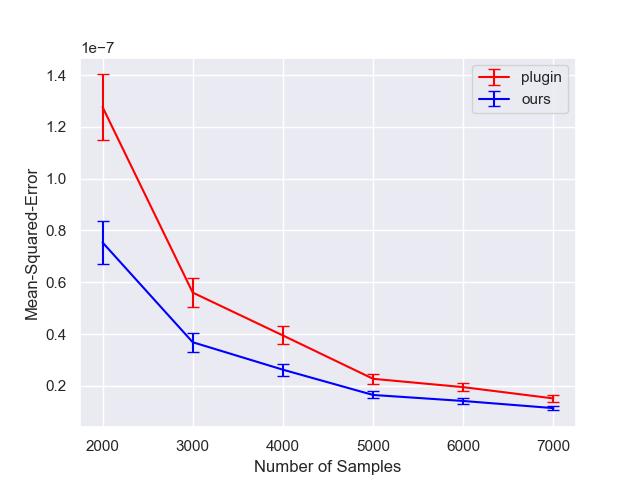
\includegraphics[width=\textwidth]{images/mse_estimators_10_bins.png}
         \caption{$B = 10$
         \pl{s/ours/canceling}
         \pl{Number of samples of what - relate to notation in text}
         \pl{label y-axis}
         }
         \label{fig:mse_estimators}
     \end{subfigure}
     \hfill
     \begin{subfigure}[b]{0.48\textwidth}
         \centering
         \includegraphics[width=\textwidth]{images/mse_estimator_100_bins.png}
         \caption{$B = 100$
         \pl{make text larger by reducing the xrange and yrange}
         }
         \label{fig:mse_vs_ce_estimators}
     \end{subfigure}
  \caption{
    Mean-squared errors of debiased (labeled as `ours') and plugin estimators on a recalibrated VGG16 model on CIFAR-10 with $90\%$ confidence intervals (lower values better). The debiased estimator is closer to the ground truth, which corresponds to $0$ on the y-axis, especially when $B$ is large and/or the number of samples $n$ is small.
}
  \label{fig:mse_estimators_bins}
\end{figure}


\begin{figure}
  \centering
  \centering
     \begin{subfigure}[b]{0.45\textwidth}
         \centering
         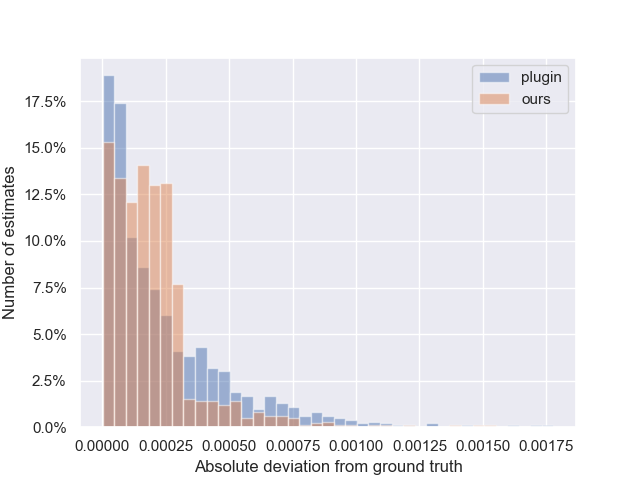
\includegraphics[width=\textwidth]{histogram_estimators_10_bins.png}
         \caption{$B$ = 10 bins}
     \end{subfigure}
     \hfill
     \begin{subfigure}[b]{0.45\textwidth}
         \centering
         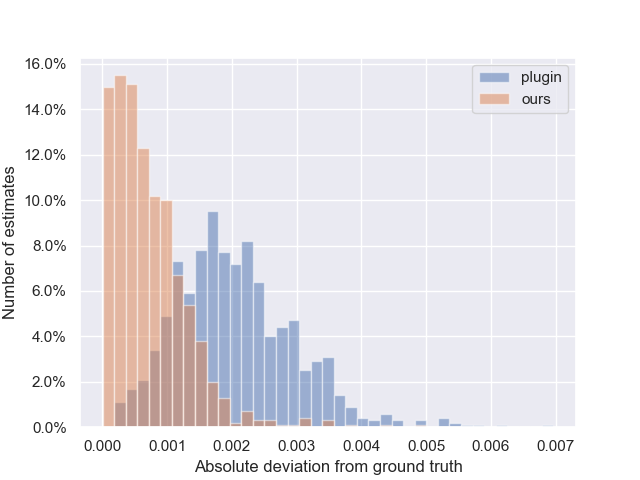
\includegraphics[width=\textwidth]{histogram_estimates_100_bins.png}
         \caption{$B = 100$ bins}
     \end{subfigure}
  \caption{Histograms of the absolute value of the difference between estimated and ground truth $\ell_2^2$ calibration errors. For $B = 10$ bins, the results are mixed but we avoid very bad estimates. For $B=100$ our estimates are much closer to ground truth.}
  \label{fig:histograms_estimators_bins}
\end{figure}

\begin{figure}
  \centering
  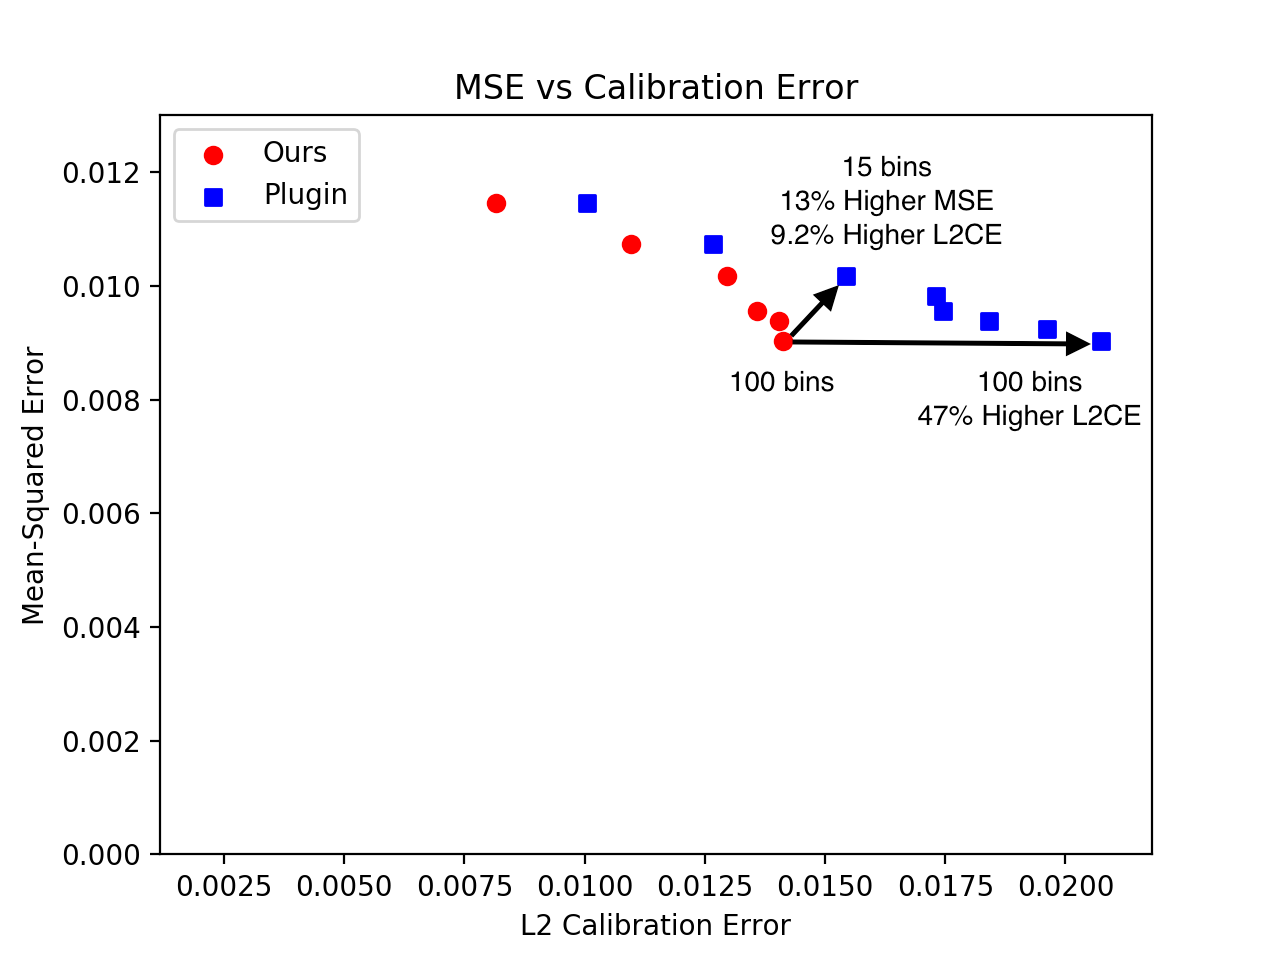
\includegraphics[width=0.9\textwidth]{mse_vs_verified_error_plugin_vs_ours.png}
  \caption{Plot of mean-squared error against 90\% upper bounds on the calibration error computed by the debiased estimator and the plugin estimator, when we vary the number of bins $B$. For a given calibration error, our estimator enables us to choose models with a better mean-squared error. If we want a model with $\ell_2$ calibration error less than 0.015, the debiased estimator tells us we can confidently use 100 bins, while relying on the plugin estimator only lets us use 15 bins and incurs a 13\% higher mean-squared error.}
  \label{fig:mse_vs_ce_estimator}
\end{figure}



\end{document}
